\documentclass[11pt, spanish]{beamer}
\usepackage{babel}
\usepackage[T1]{fontenc}
\usepackage[utf8]{inputenc}

\usepackage{pgf,pgfpages}
\usepackage{pgffor} % For loops

\usepackage{tikz}
\usetikzlibrary{arrows,shapes,backgrounds,calc}

\usepackage{graphicx}
\usepackage{colortbl}
\usepackage{units}

% \usepackage{calrsfs}bab
% \DeclareMathAlphabet{\pazocal}{OMS}{zplm}{m}{n}
% \usepackage{calligra}
\usepackage[cal=boondox,scaled=1.15]{mathalfa}
% \usepackage{bickham}
% \usepackage{boondox-cal}
% \usepackage{boondox-calo}
% \usepackage{dutchcal}

%% Beamer style >>>>>>>>>>>>>>>>>>>>>>>>>
\mode<presentation>
{
  \usetheme{PHD}
  \setbeamercovered{transparent}
  \setbeamertemplate{items}[square]
}

%\usefonttheme[onlymath]{serif}

\beamertemplatenavigationsymbolsempty

\defbeamertemplate{enumerate item}{mycircle}
{
  %\usebeamerfont*{item projected}%
  \usebeamercolor[bg]{item projected}%
  \begin{pgfpicture}{0ex}{0ex}{1.5ex}{0ex}
    \pgfcircle[fill]{\pgfpoint{-0.1pt}{.65ex}}{1.1ex}
    \pgfbox[center,base]{\color{PHDyellowd}{\insertenumlabel}}
  \end{pgfpicture}%
}
[action]
{\setbeamerfont{item projected}{size=\scriptsize}}
\setbeamertemplate{enumerate item}[mycircle]

\setbeamertemplate{frametitle continuation}[from second][] % No automatic symbols I II II
%<<<<<<<<<<<<< beamer style

\title{Redes Neuronales y otros Artefactos Matemáticos\vspace{-0.5em}}
\author[J.R. Rodr\'{\i}guez Galv\'an]{\em\structure{Daniel Acosta Soba, Noelia Ortega Román, Álex Pérez Fernández, Rafa Rodríguez Galván}\vspace{-1.5em}}
\date{\scriptsize{Facultad de Ciencias, Universidad de C\'adiz}\\[0.9em]\small Día Internacional de las Matemáticas («día {\Huge$\pi$}»), 2023}

% XeLaTeX font choosing
% \usepackage{fontspec}%{xltxtra} %fontspec}
% \setsansfont{Fontin Sans}
% \setsansfont{Lato}

% PDFLaTeX font choosing
\usepackage[default, scale=1.0]{lato}


% \usepackage{array, multirow, rotating} % booktabs: toprule, midrule...
\usepackage{array,booktabs,tabularx}

\usepackage{current-definitions}

\newtheorem{remark}{Remark}
\newtheorem{proposition}{Proposition}
%\newtheorem{theorem}{Theorem}

% Presentation goodies >>>>>>>>>>>>>>>>>>>>>>>>>>>>
\newcommand<>{\myframed}[1]{\alt#2{\tikz[phd] \node[box] {#1};}{{#1}}}
\newcommand<>{\myframedAlert}[1]{\alt#2{\tikz[phdB] \node[boxB] {\color{black}#1};}{{#1}}}
\newcommand<>{\framedmath}[1]{%
\alt#2{\tikz[phd] \node[box] {\ensuremath{#1}};}{\ensuremath{#1}}}
\newcommand{\framedB}[1]{\tikz[phd] \node[boxB] {#1};}
\newcommand{\framedmathB}[1]{\framedB{\ensuremath{\displaystyle{#1}}}}
\newcommand{\ver}[1]{\footnote{See #1}}
\newcommand{\cita}[1]{{\color{PHDgray}\cite{#1}}}
\newcommand\cellalert[2]{\only<#1>{\cellcolor{PHDyellow}}\alt<#1>{\textbf{#2}}{#2}}
\newcommand{\soften}[1]{{\color{PHDgray}#1}}
\newcommand{\rowalert}[7]{%
    \cellalert{#1}{#2} & \cellalert{#1}{#3} &
    \cellalert{#1}{#4} & \cellalert{#1}{#5} &
    \cellalert{#1}{#6} & \cellalert{#1}{#7}}

% \usepackage{wasysym}
% \newcommand{\good}{{\color{PHDgreen}$\CIRCLE$}} %\blacksmiley
% \newcommand{\bad}{{\color{PHDred}$\CIRCLE$}}
\usepackage{pifont, fontawesome}
\newcommand{\good}{{\color{PHDgreen}\ding{52}}}
\newcommand{\bad}{{\color{PHDred}\ding{56}}}
\newcommand{\exclamation}{{\large\color{PHDred}{\textbf{\itshape !}}}}
\newcommand{\question}{{\large\color{PHDred}{\textbf{\itshape ?}}}}
\newcommand\colorUnderLine[2][PHDyellow]{\color{#1}\underline{{\color{black}#2}}\color{black}\xspace}
\newcommand\gris[1]{{\color{PHDgray}#1}}
\newcommand\amarillo[1]{{\color{PHDyellow}#1}}
\newcommand\tiragris[1]{{\par\hfill\small\gris{#1}}}
\newcommand\point{\alert{\faHandORight}\xspace}
%<<<<<<<<<<<<<<<

\setcounter{tocdepth}{1}


%
% Bibliography
%
%\usepackage{natbib}

% To list each bibliographic entry in a line
\setbeamertemplate{bibliography entry title}{}
\setbeamertemplate{bibliography entry location}{}
\setbeamertemplate{bibliography entry note}{}

% ... end of preamble.

\AtBeginSection{\frame{\sectionpage}}

\colorlet{inputcolor}{green!60!black}
\colorlet{hiddencolor}{blue!60!black}
\colorlet{outcolor}{red!60!black}

%======================================================================
\begin{document}
%======================================================================

% Tikz style and beamer template ------->>>
\tikzstyle{every picture}+=[remember picture]
\tikzstyle{na} = [baseline=-.5ex]
\tikzstyle{phd} = [baseline=-.6ex,
  box/.style={rectangle, draw=PHDblueC, thick, fill=PHDblueA,
    align=center, rounded corners, minimum height=1.6em},
  boxB/.style={rectangle, draw=PHDredA, thick, fill=PHDblueA,
    align=center, rounded corners, minimum height=1.6em}]
\tikzstyle{phdB} = [baseline=-.7ex,
  box/.style={rectangle, draw=PHDblueC, thick, fill=PHDblueA,
    align=center, rounded corners, minimum height=1.6em},
  boxB/.style={rectangle, draw=PHDredA, thick, fill=PHDblueA,
    align=center, rounded corners, minimum height=1.6em}]
\tikzstyle{myarrow} = [->,>=latex, PHDredA, shorten >=4pt,
  opacity=.6, line width=0.6mm]
\tikzstyle{myarrow2} = [->,>=latex, PHDblueC, shorten >=4pt, opacity=.2, line width=0.4mm]
\tikzstyle{myarrow3} = [
     opacity=.7,
%    >=triangle 60,              % Nice arrows; your taste may be different
    node distance=6mm and 60mm, % Global setup of box spacing
    every join/.style={norm},   % Default linetype for connecting
                                % boxes
    line width=0.6mm,
    PHDredA,
    ->
    ]
\setbeamertemplate{background}
 {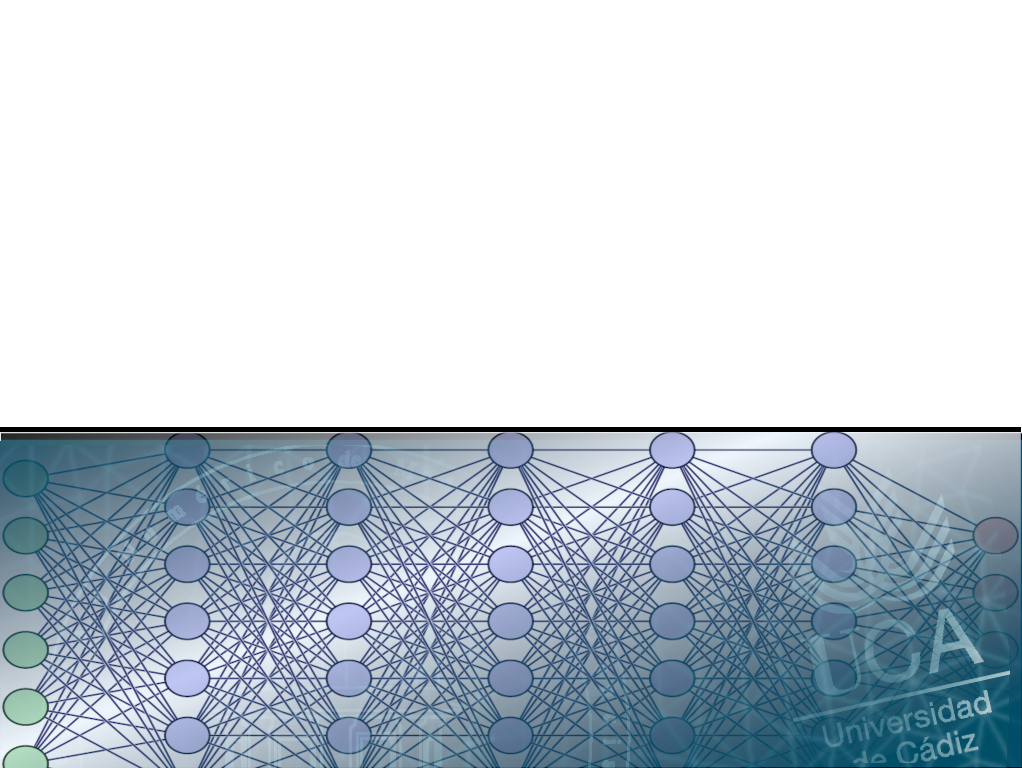
\includegraphics[width=\paperwidth,height=\paperheight]{frontpage_bg}}
\setbeamertemplate{footline}[default]
% <<<-------


% Write custom titlepage ------->>>
\begin{frame}
  \titlepage
  \vspace{5cm}
\end{frame}

% Set the background for the rest of the slides.
\setbeamertemplate{background}{}
 % {
\includegraphics[width=\paperwidth,height=\paperheight]{slide_bg}}


% Write all of the slides..........

% \begin{frame}{Outline}
%   \tableofcontents
% \end{frame}

% Start inserting infoline at the end
\setbeamertemplate{footline}[PHDtheme]
% <<<-------

\newcommand{\imgdir}{Undefined, use renewcommand!}

%============================================================================
\section{Redes Neuronales}
%============================================================================

%=====================================================================
\begin{frame}{Las redes neuronales...}
%---------------------------------------------------------------------
  \vspace{-0.9em}
  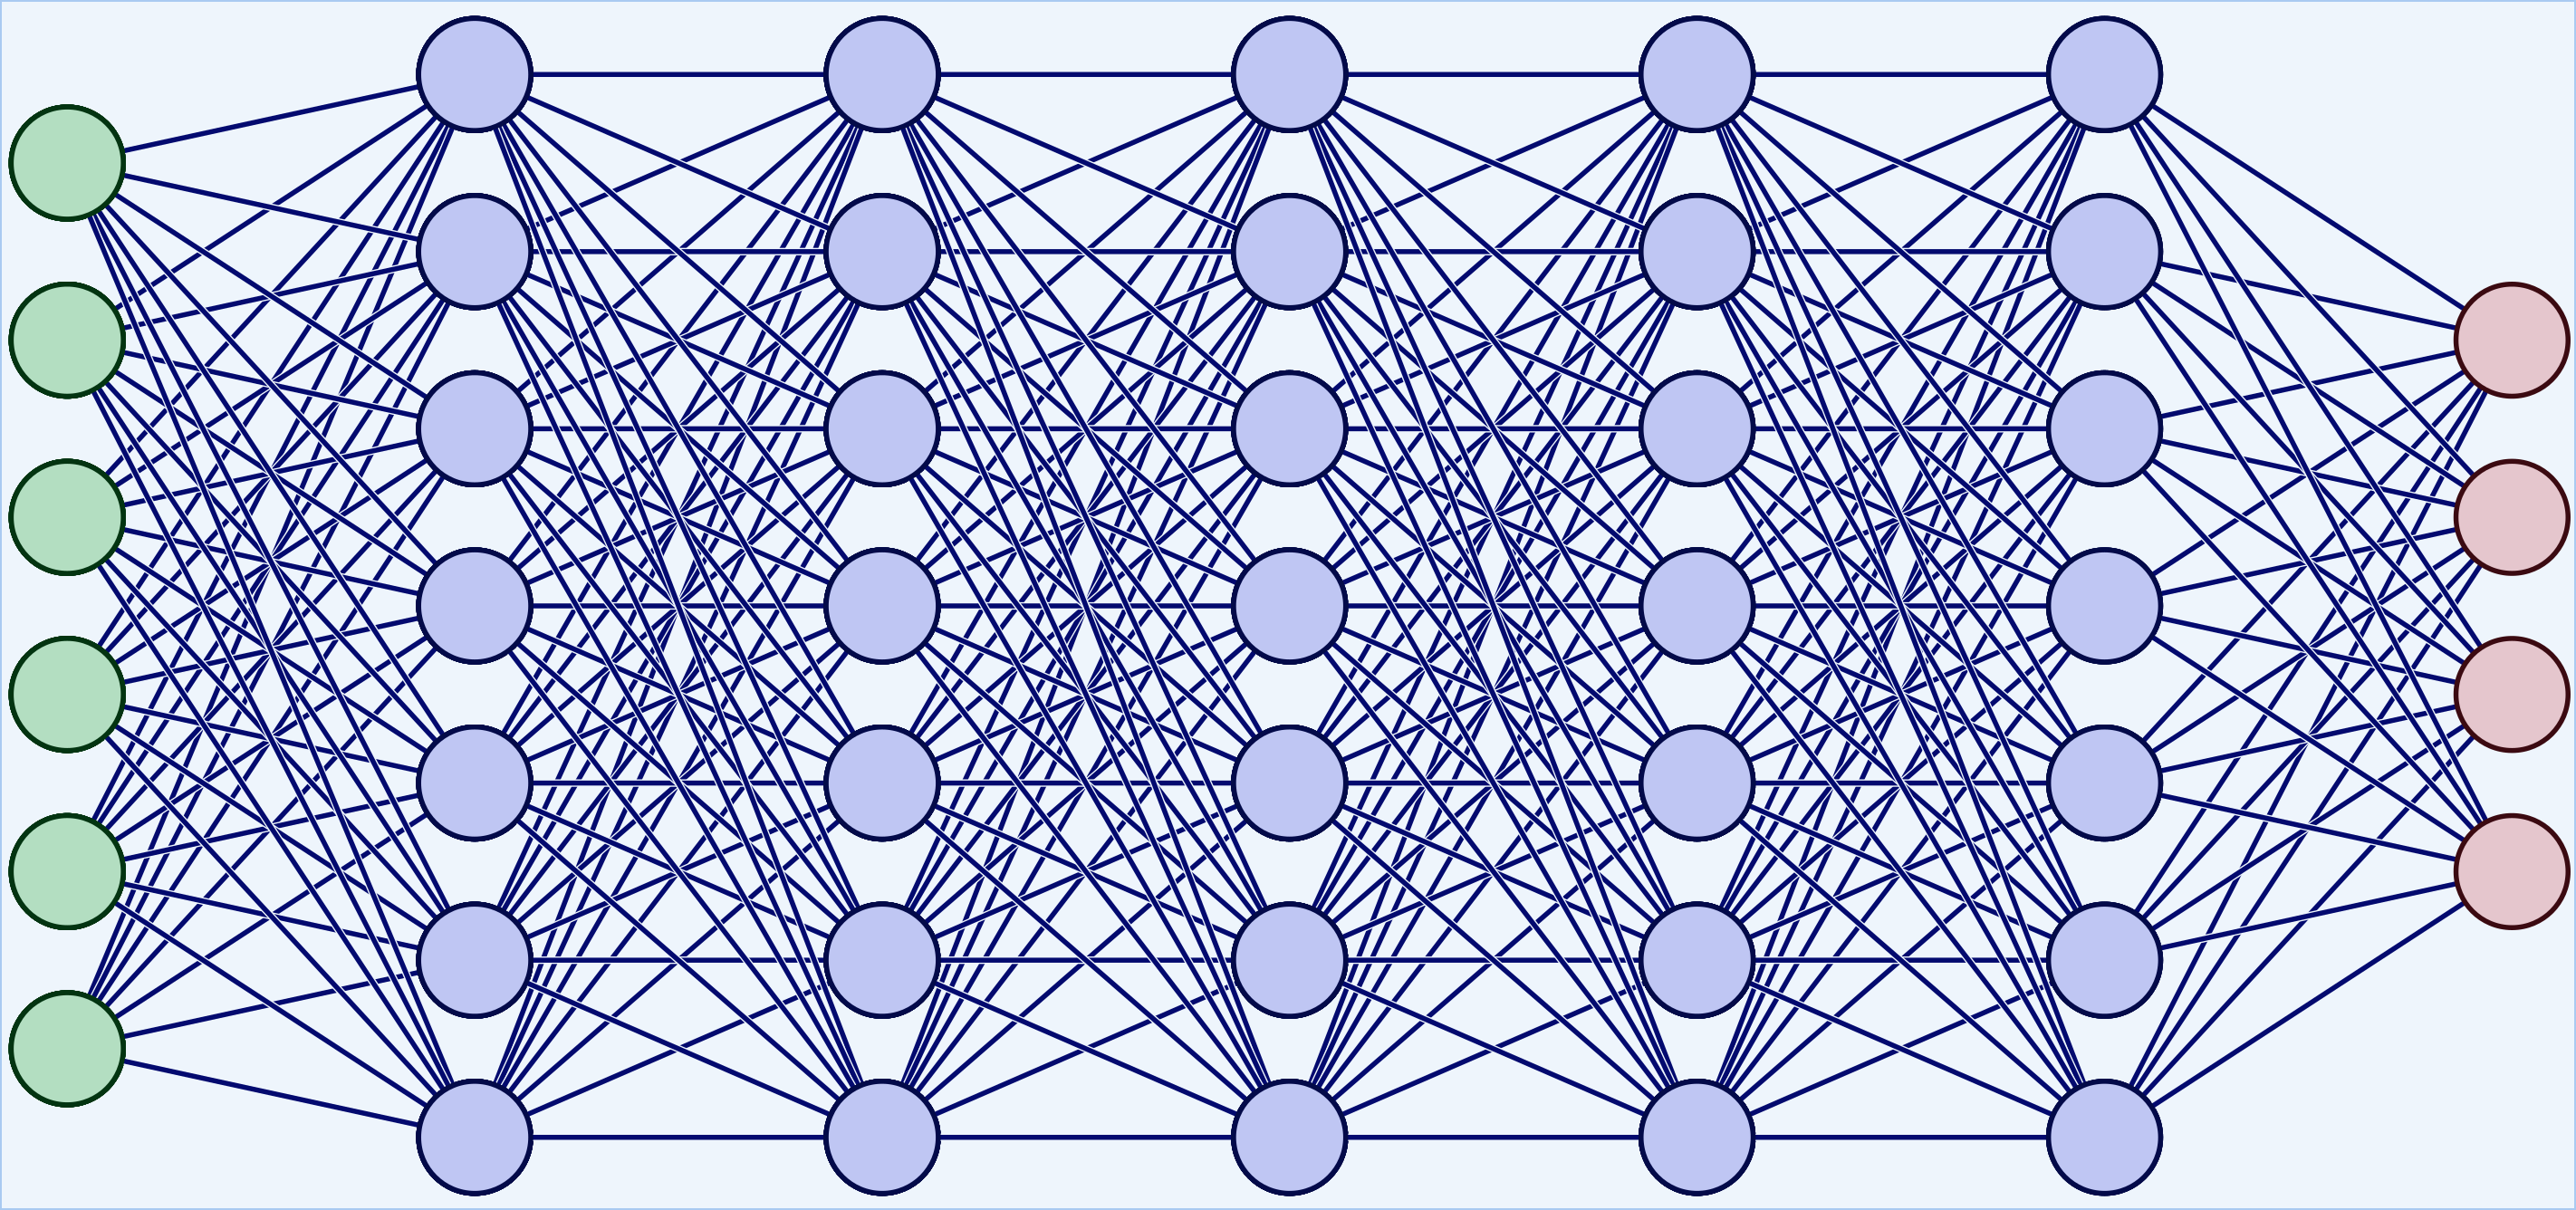
\includegraphics[width=0.95\linewidth]{deep-NN}
  \pause
  ~
  \vfill
  {\large\textbf{...son artefactos matemáticos:}}
  \begin{gather*}
    {\color{inputcolor} \xx} \mapsto 
    {\color{hiddencolor}\ff_1({\color{inputcolor} \xx})} \mapsto \pause
    {\color{hiddencolor}\ff_2\circ \ff_1({\color{inputcolor} \xx})} \mapsto \pause
    % {\color{hiddencolor}\ff_3\circ \ff_2\circ \ff_1({\color{inputcolor} x})} \mapsto \pause
    {\color{hiddencolor} \cdots} \mapsto
    {\color{hiddencolor} \ff_L\circ \cdots \circ \ff_2\circ \ff_1({\color{inputcolor} x})} = {\color{outcolor}\mathbf{y}}
  \end{gather*}
\end{frame}

\begin{frame}
  \vspace{-0.2em}
  \begin{flushright}
  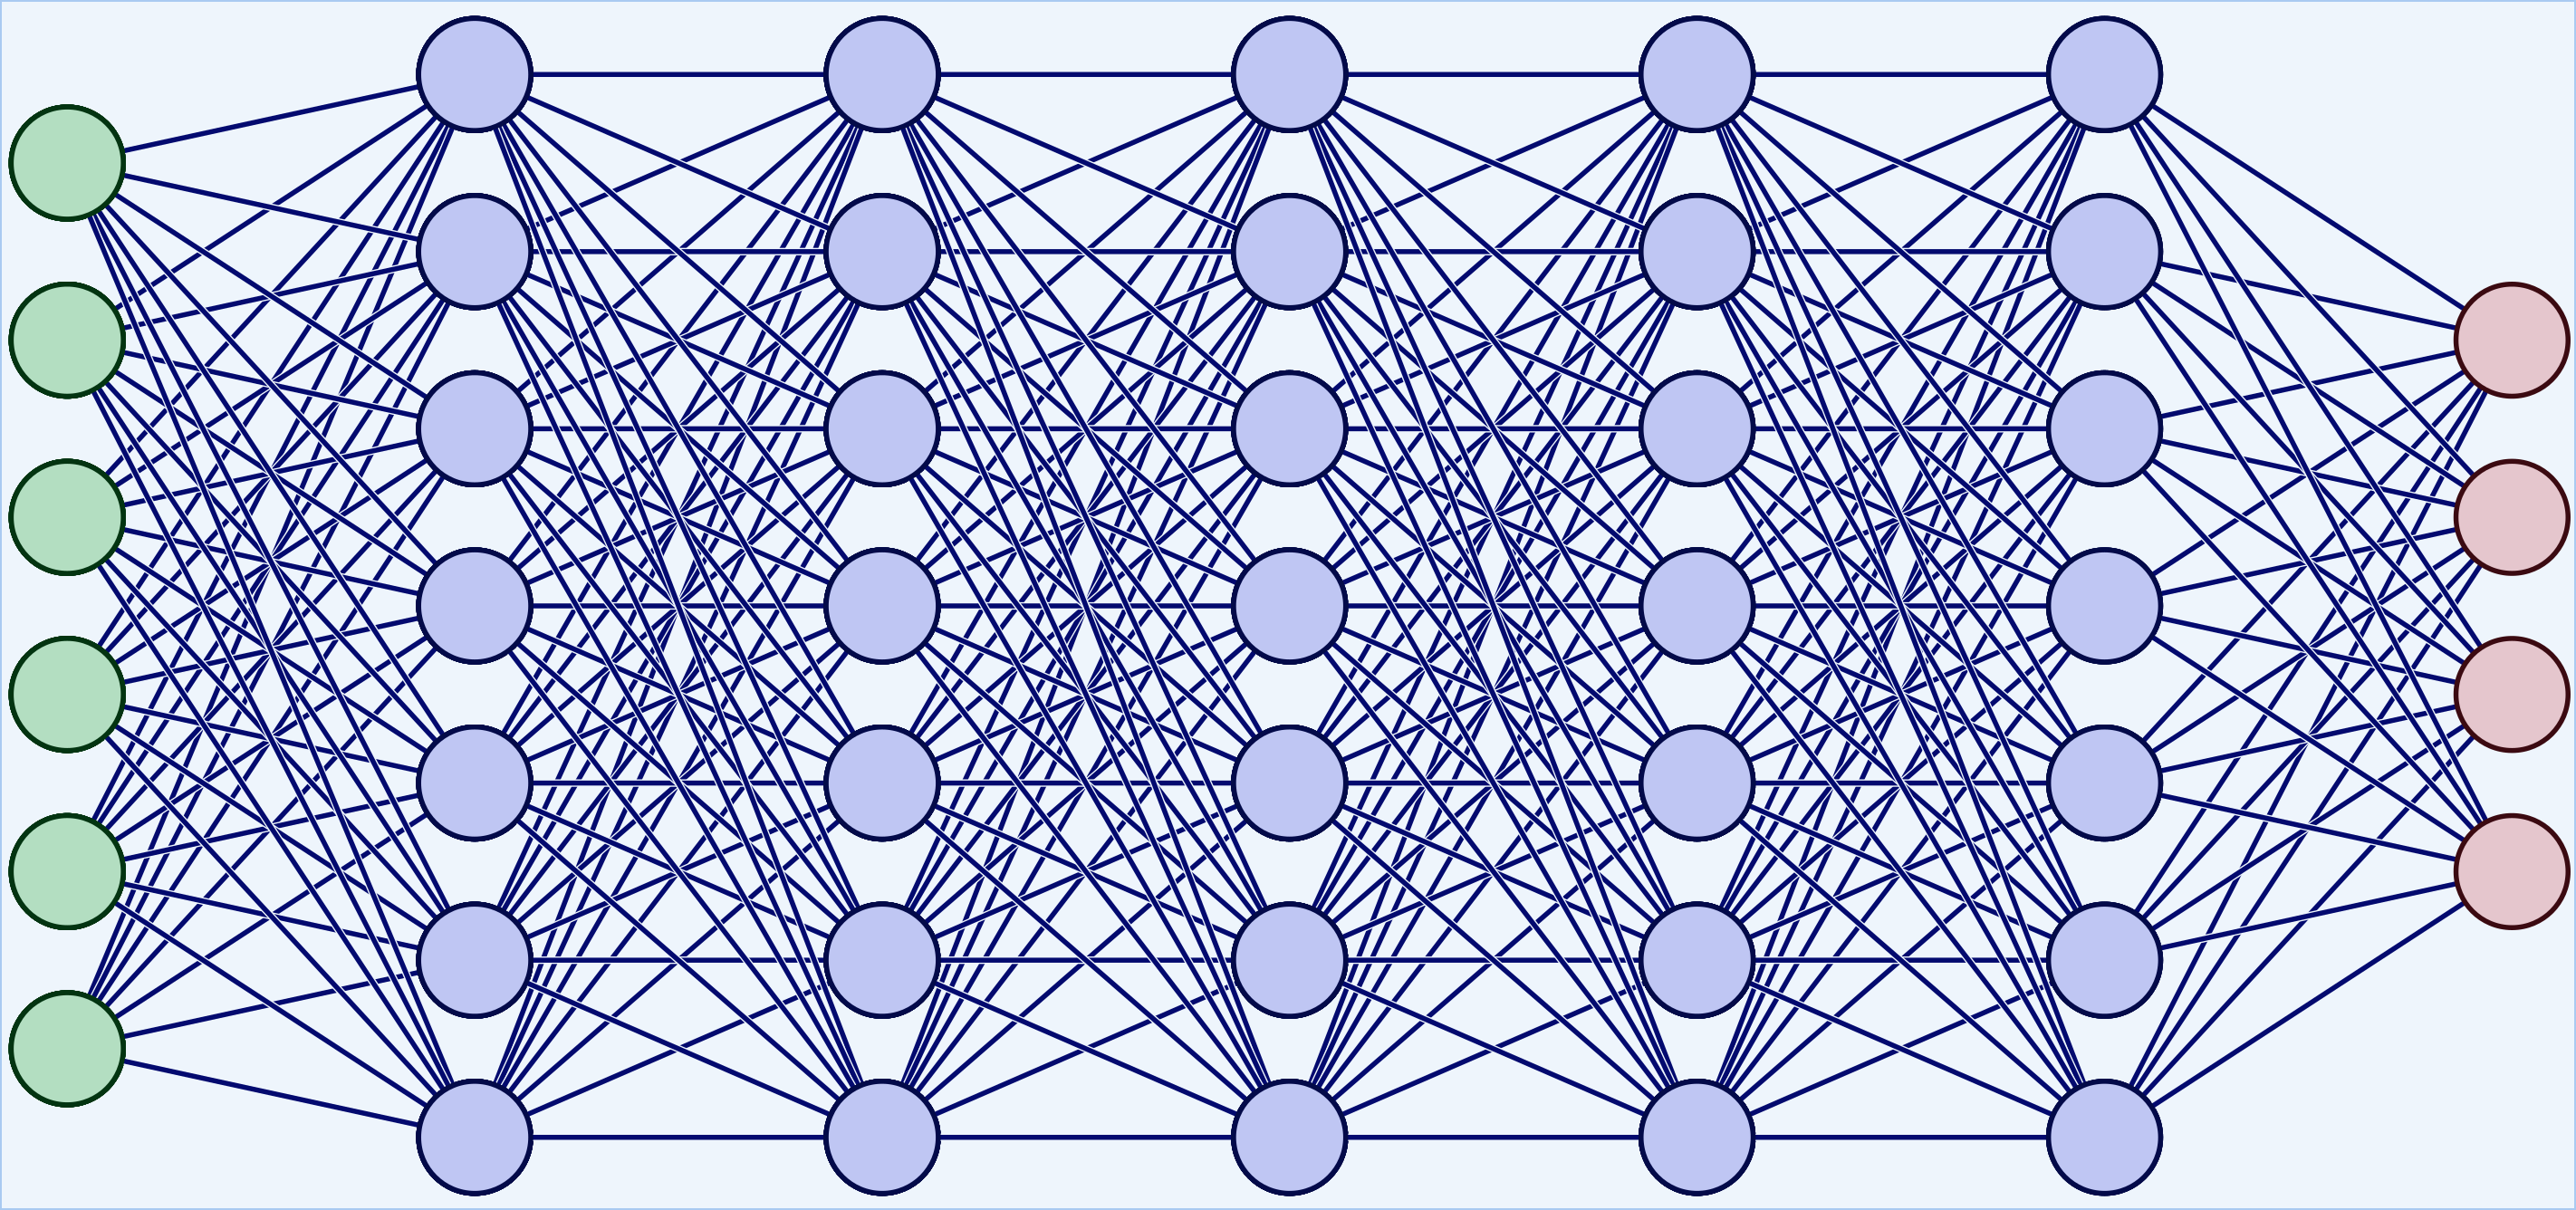
\includegraphics[width=0.52\linewidth]{deep-NN}
  \end{flushright}
  \vspace{-0.7em}
  {\large\textbf{Definición}}:\par
  una \structure{\bf Red Neuronal} (\textit{RN} o \textit{NN}) es una función $f_{NN}:\Rset^n \to \Rset^m$ del tipo:
    $$
    {\color{outcolor}\mathbf{y}} = f_{NN}({\color{inputcolor}x}) = 
    {\color{hiddencolor} \ff_L\circ \cdots \circ \ff_2\circ \ff_1({\color{inputcolor} x})}.
    $$
  Donde...
  \begin{itemize}
    \item Cada función $\ff_i$ se llama una \textbf{capa} (oculta)
    \item Cada capa $\ff_i$ está compuesta por un nº variable de \textbf{neuronas}
    \item Cada neurona (y por tanto cada capa) depende un conjunto de \textbf{parámetros}, que determinarán a la RN 
  \end{itemize} 
  \bigskip
  \scriptsize
  \begin{flushright}
  $\star$ La RN de la figura  se dice de tipo «\textit{feed forward}» o {prealimentada}
  \end{flushright}
\end{frame}

\begin{frame}{Un ejemplo}
  \vspace{-0.5em}
  \begin{center}
  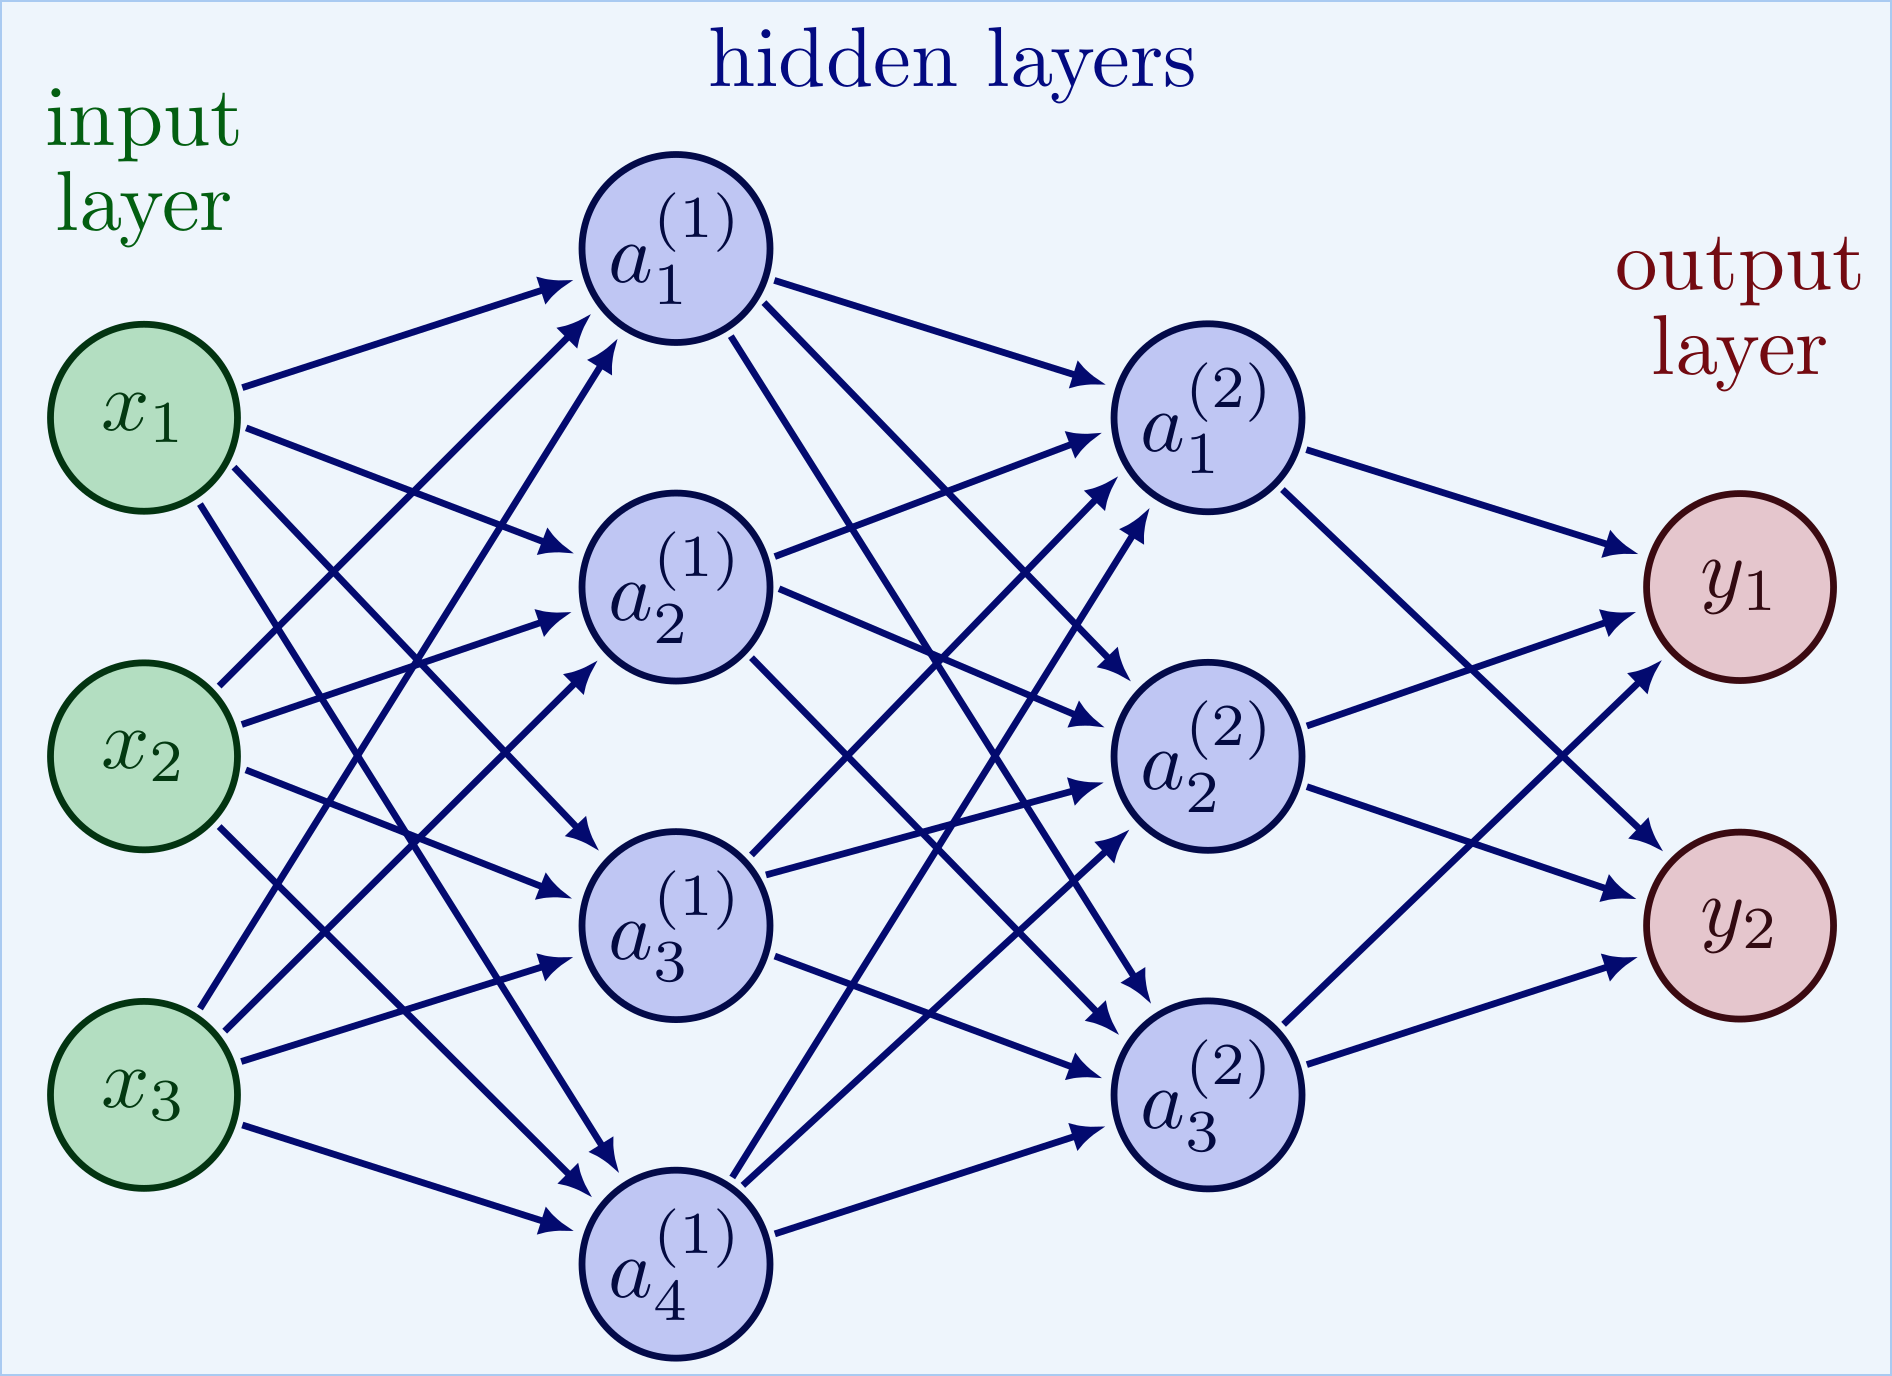
\includegraphics[width=0.82\linewidth]{example-NN}
  \end{center}
  $$
  f_{NN}:\Rset^3 \to \Rset^2
  \mbox{con $2$ capas ocultas de $4$ y $3$ neuronas}
  $$
\end{frame}


\begin{frame}{Neurona o \emph{perceptrón} simple}
  Cada neurona $j$ de una capa oculta $f_i$ (o de salida $y_i$) es una función% 
  \footnote{Donde $N_i$ es el número de neuronas de la capa $i-1$}:
  $$
  \xx\in \Rset^{N_{i}} \rightarrow \alert{a_j^{(i)}}(\xx) \in \Rset,
  $$
  composición de%
  \begin{itemize}
    \item una función afín con parámetros $\structure{\ww}=({w_1},\dots,{w_{N_i}})$ y \structure{$b$}
    \item una función no lineal $\sigma$, llamada «\structure{función de activación}»  
  \end{itemize}
  \begin{block}{}
    \vspace{-0.8em}
  \begin{align*}
    \alert{a_j^{(i)}}(\xx) &= \sigma(w_1 x_1 + w_2 x_2 + \cdots + w_{N_i} x_{N_i} + b) = \\
                   &=\sigma\Big(\sum_{k=1}^{N_i} w_k x_k +b\Big) = \sigma(\ww\cdot\xx + b)
  \end{align*}
  \end{block}
\end{frame}

\begin{frame}{Con más propiedad...}
Para aligerar la notación se omitieron los índices correspondientes a la capa, $i$, y a la neurona, $j$. Debería ser:
  \begin{align*}
    \alert{a_j^{(i)}}(\xx) = \sigma\Big(\sum_{k=1}^{N_i} w^{(i)}_{j,k} x_k +b^{(i)}_j\Big).
    % = \sigma\big(\ww^{(i)}\cdot\xx + b^{(i)}_j\big)
  \end{align*}
  Así, si $\WW^{(i)}$ denota a la matriz de valores $w^{(i)}_{j,k}$, y $\vect b^{(i)}$ es el vector $(b^{(i)}_j)$, podemos escribir a tod la \alert{capa} $i$ como:
$$
\alert{\ff_i(\xx)} = {\boldsymbol\sigma_i}(\WW^{(i)}\xx + \vect b^{(i)})
$$
La RN está determinada por los parámetros $\WW^{(i)}$, los desplazamientos $\vect b^{(i)}$ y las funciones de activación $\boldsymbol\sigma_i$
\end{frame}

\begin{frame}{Funciones de activación}
  \vspace{-0.7em}
  \begin{center}
  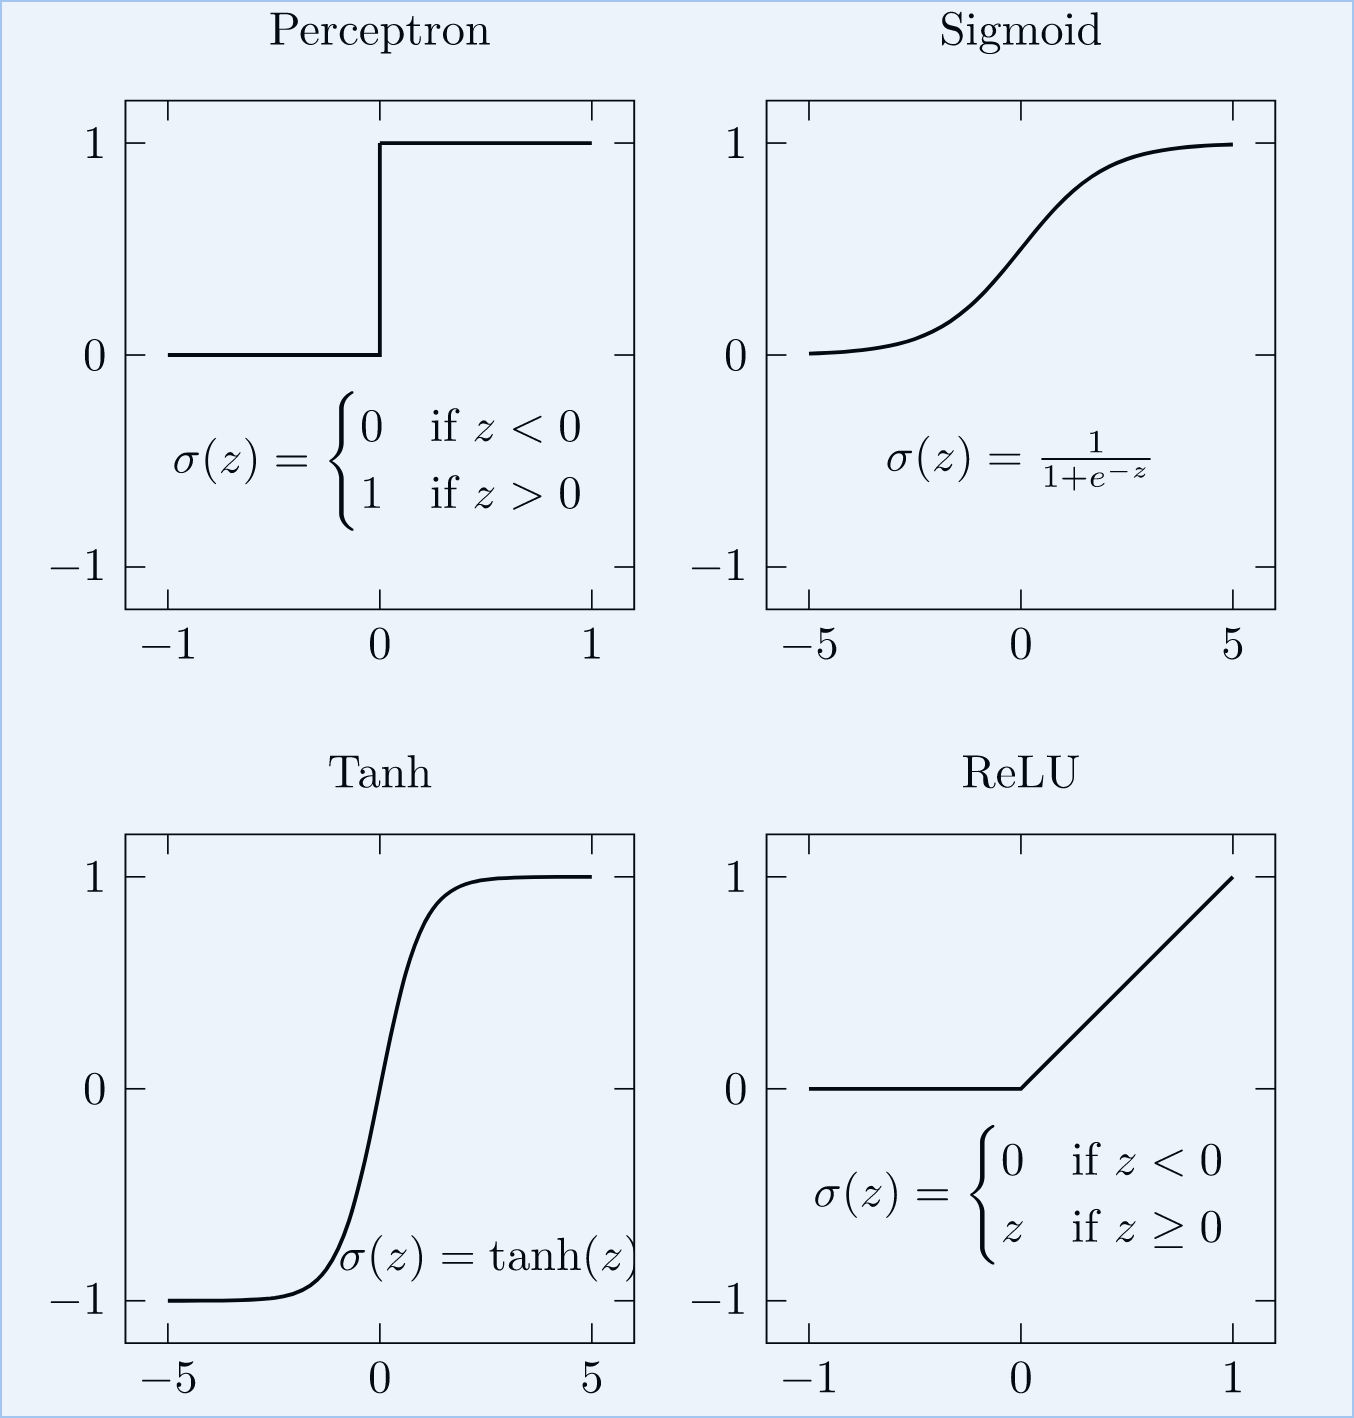
\includegraphics[width=0.65\linewidth]{funciones_activacion}
  \end{center}
\end{frame}

%============================================================================
\section{Ajuste de los parámetros}
%============================================================================


\include{dan1}

%% Beamer style >>>>>>>>>>>>>>>>>>>>>>>>>

\setbeamertemplate{enumerate item}[mycircle]

\setbeamertemplate{frametitle continuation}[from second][] % No automatic symbols I II II
%<<<<<<<<<<<<< beamer style

%\title{Redes Neuronales y otros Artefactos Matemáticos\vspace{-0.5em}}
%\author[J.R. Rodr\'{\i}guez Galv\'an]{\em\structure{Daniel Acosta Soba, Noelia Ortega Román, Álex Pérez Fernández, Rafa Rodríguez Galván}\vspace{-1.5em}}
%\date{\scriptsize{Facultad de Ciencias, Universidad de C\'adiz}\\[0.9em]\small Día Internacional de las Matemáticas («día {\Huge$\pi$}»), 2023}

% XeLaTeX font choosing
% \usepackage{fontspec}%{xltxtra} %fontspec}
% \setsansfont{Fontin Sans}
% \setsansfont{Lato}


\setcounter{tocdepth}{1}
\newcommand{\Olf}{\mathcal{O}}
\newcommand{\SVZdomain}{\text{\it SVZ}}
\newcommand{\NZdomain}{\text{\it NZ}}
\newcommand{\CCdomain}{{\text{\it CC}}}
\newcommand{\CCexp}{\mu_{CC}}
\newcommand{\tCCexp}{\tilde{\mu}_{CC}}
\def\SO{\sigma}
\def\X{\chi}
\def\D{\mathscr{D}}
\def\T{\mathcal{T}}
\def\E{\mathcal{E}}
\def\S{\mathcal{S}}
\def\N{\mathbb{N}}
\def\P{\mathbb{P}}
\def\O{\mathcal{O}}

%
% Bibliography
%
%\usepackage{natbib}

% To list each bibliographic entry in a line
\setbeamertemplate{bibliography entry title}{}
\setbeamertemplate{bibliography entry location}{}
\setbeamertemplate{bibliography entry note}{}

% ... end of preamble.

\AtBeginSection{\frame{\sectionpage}}

\colorlet{inputcolor}{green!60!black}
\colorlet{hiddencolor}{blue!60!black}
\colorlet{outcolor}{red!60!black}

%======================================================================

%======================================================================

% Tikz style and beamer template ------->>>
\tikzstyle{every picture}+=[remember picture]
\tikzstyle{na} = [baseline=-.5ex]
\tikzstyle{phd} = [baseline=-.6ex,
  box/.style={rectangle, draw=PHDblueC, thick, fill=PHDblueA,
    align=center, rounded corners, minimum height=1.6em},
  boxB/.style={rectangle, draw=PHDredA, thick, fill=PHDblueA,
    align=center, rounded corners, minimum height=1.6em}]
\tikzstyle{phdB} = [baseline=-.7ex,
  box/.style={rectangle, draw=PHDblueC, thick, fill=PHDblueA,
    align=center, rounded corners, minimum height=1.6em},
  boxB/.style={rectangle, draw=PHDredA, thick, fill=PHDblueA,
    align=center, rounded corners, minimum height=1.6em}]
\tikzstyle{myarrow} = [->,>=latex, PHDredA, shorten >=4pt,
  opacity=.6, line width=0.6mm]
\tikzstyle{myarrow2} = [->,>=latex, PHDblueC, shorten >=4pt, opacity=.2, line width=0.4mm]
\tikzstyle{myarrow3} = [
     opacity=.7,
%    >=triangle 60,              % Nice arrows; your taste may be different
    node distance=6mm and 60mm, % Global setup of box spacing
    every join/.style={norm},   % Default linetype for connecting
                                % boxes
    line width=0.6mm,
    PHDredA,
    ->
    ]
\setbeamertemplate{background}
 {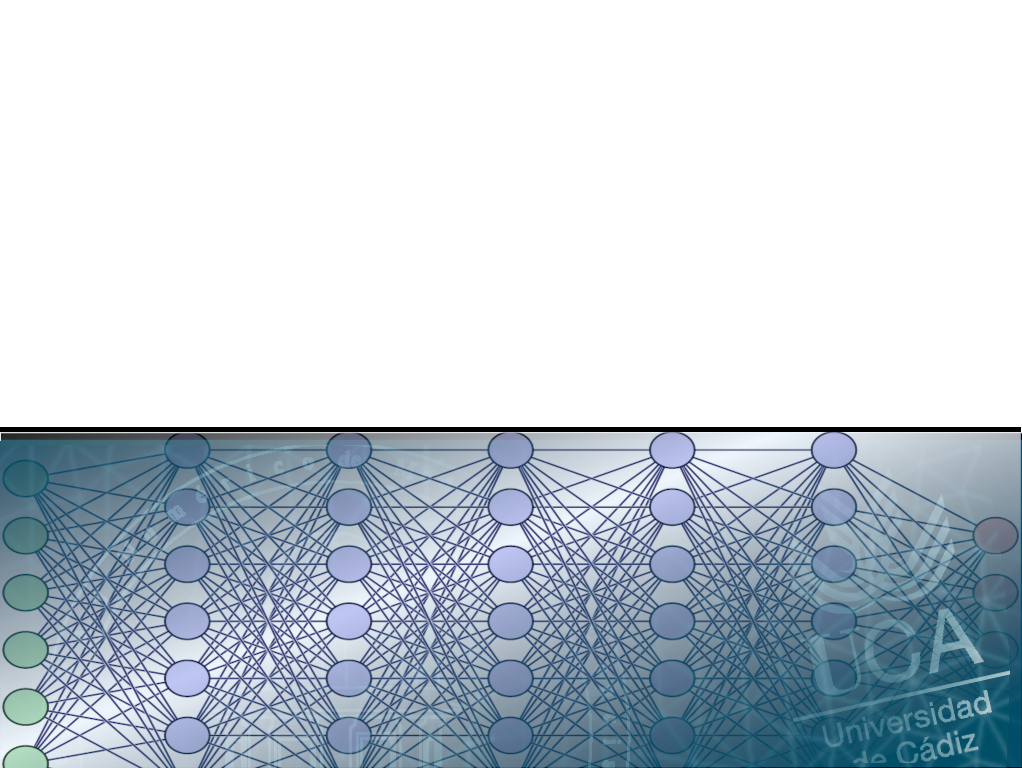
\includegraphics[width=\paperwidth,height=\paperheight]{frontpage_bg}}
\setbeamertemplate{footline}[default]
% <<<-------


% Write custom titlepage ------->>>
%\begin{frame}
%  \titlepage
%  \vspace{5cm}
%\end{frame}

% Set the background for the rest of the slides.
\setbeamertemplate{background}{}
 % {
\includegraphics[width=\paperwidth,height=\paperheight]{slide_bg}}


% Write all of the slides..........

% \begin{frame}{Outline}
%   \tableofcontents
% \end{frame}

% Start inserting infoline at the end
\setbeamertemplate{footline}[PHDtheme]
% <<<-------

%\newcommand{\imgdir}{Undefined, use renewcommand!}

%============================================================================
\section{Migración de neuroblastos en el cerebro adulto}
%============================================================================

%=====================================================================
\begin{frame}{¿Qué queremos modelar?}
%---------------------------------------------------------------------
\only<1>{
  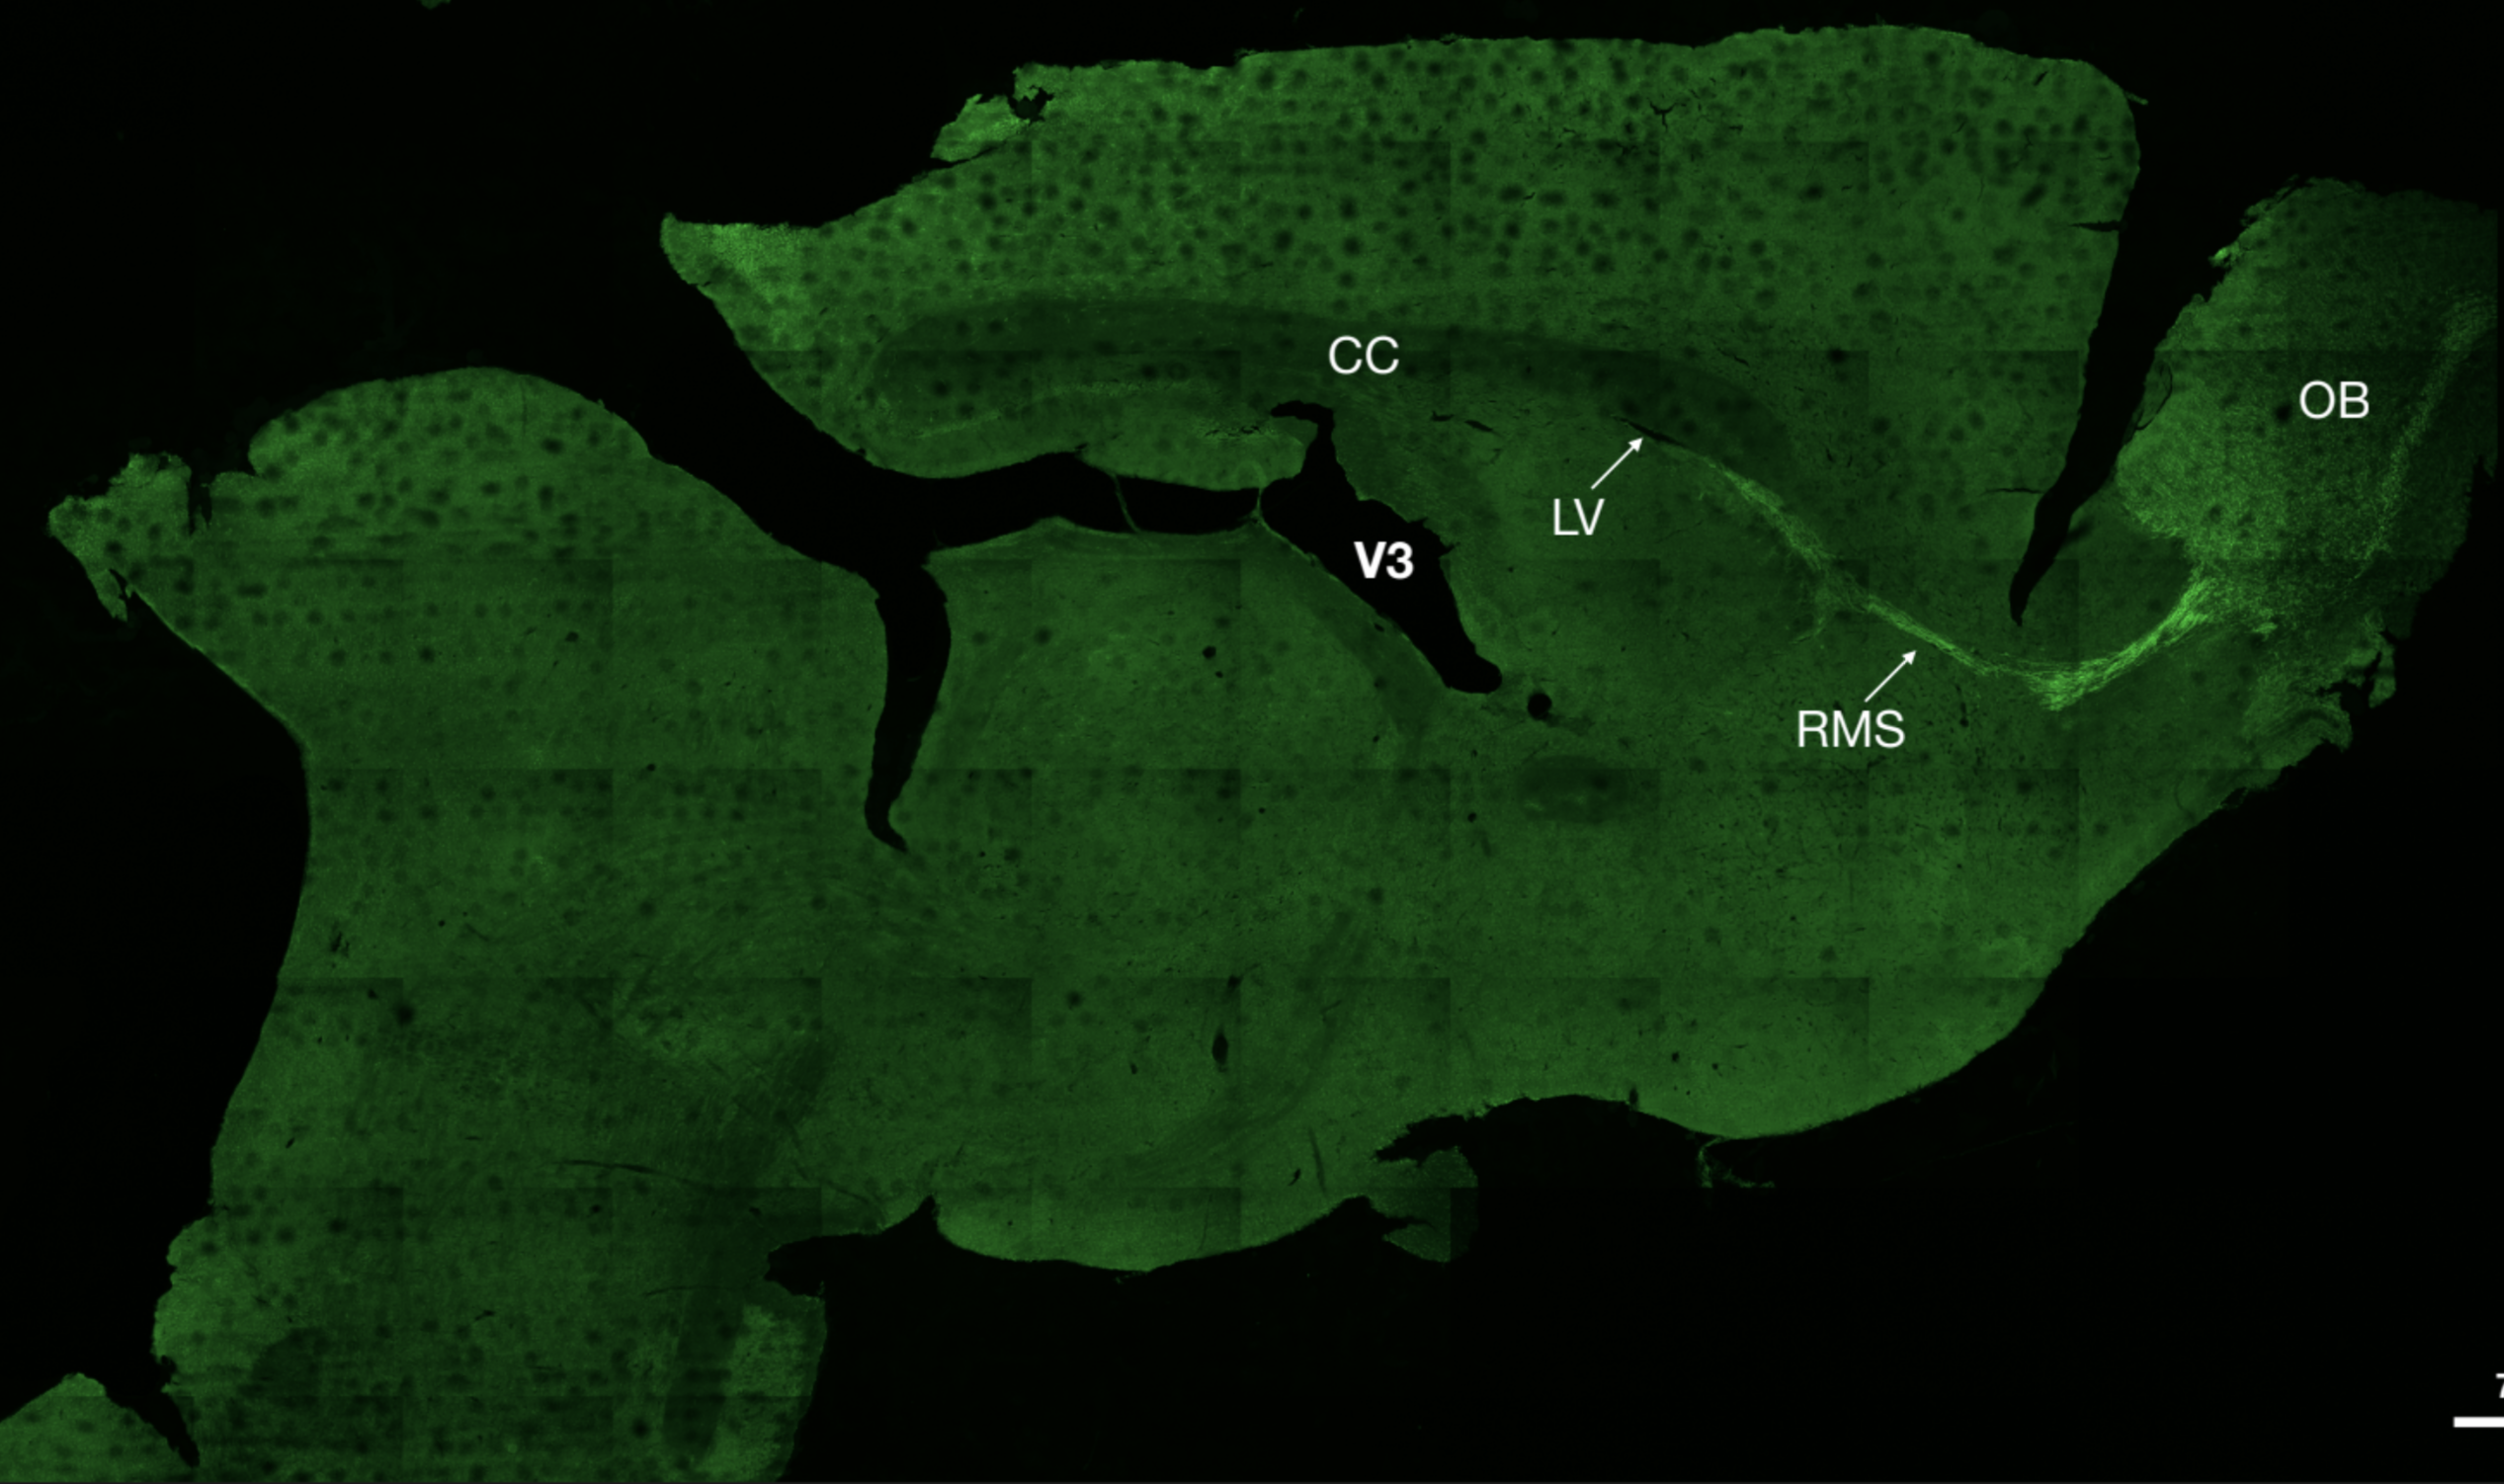
\includegraphics[width=0.95\linewidth]{cerebro-completo}}
  \only<2->{
  \includegraphics[width=0.95\linewidth]{via-rostral}}
\end{frame}

\begin{frame}{Primer objetivo: recuento de neuroblastos}
  \only<1>{
  	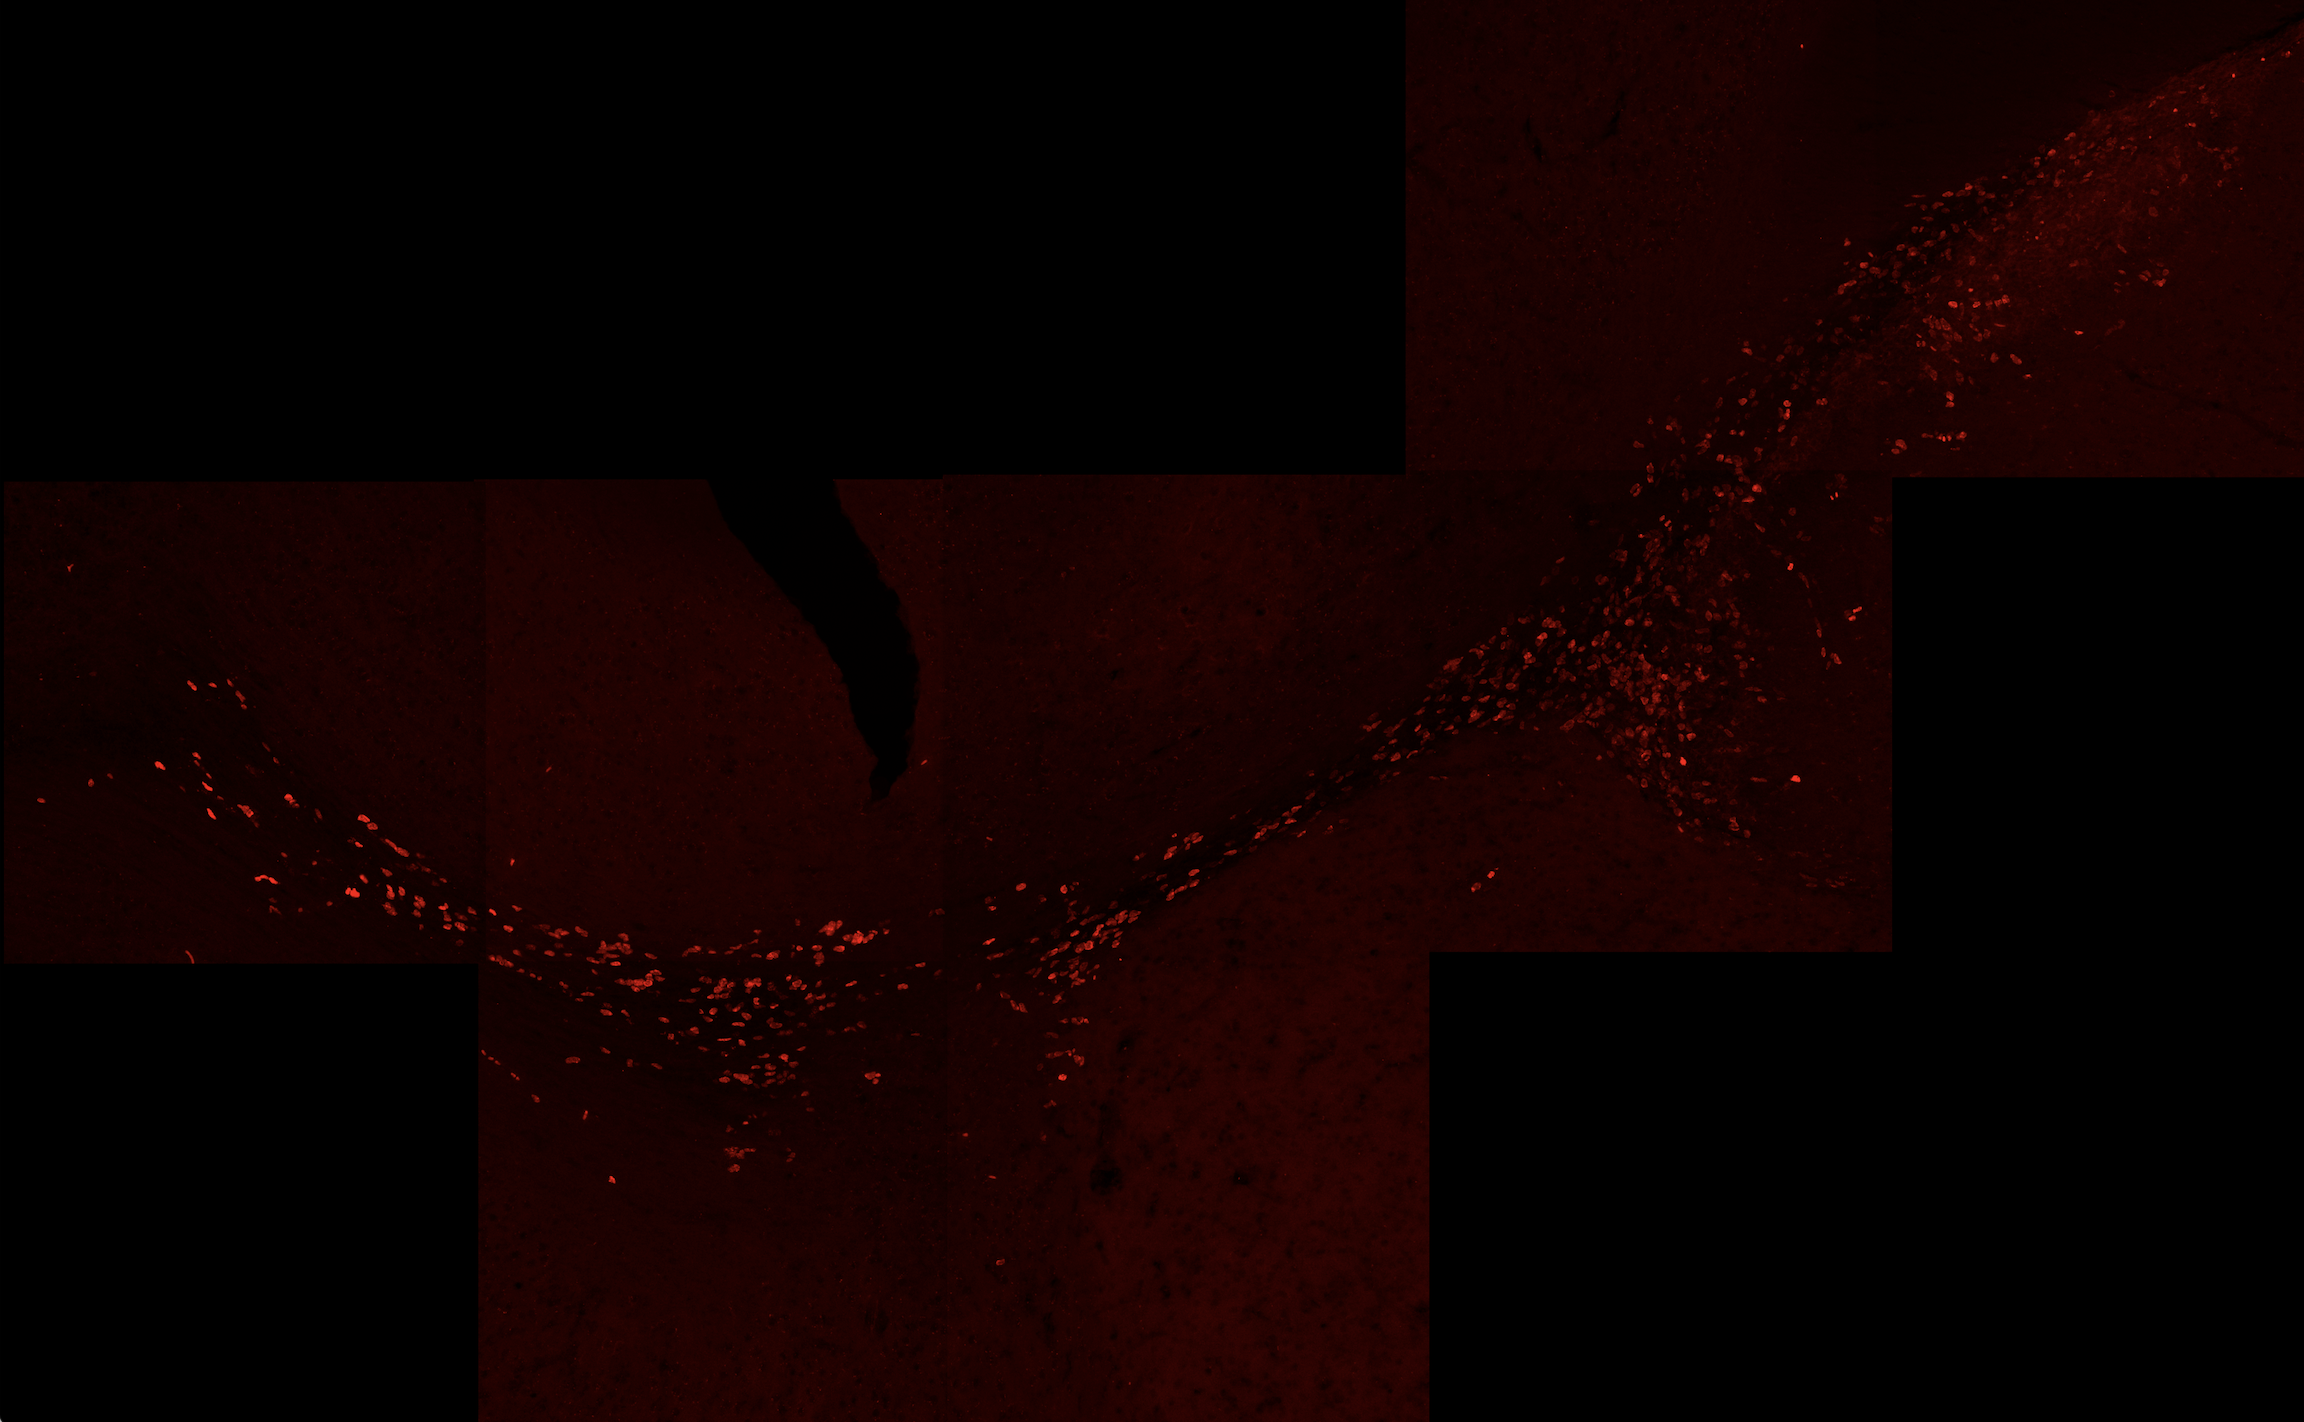
\includegraphics[width=0.95\linewidth]{via-roja}}
  \only<2->{
  	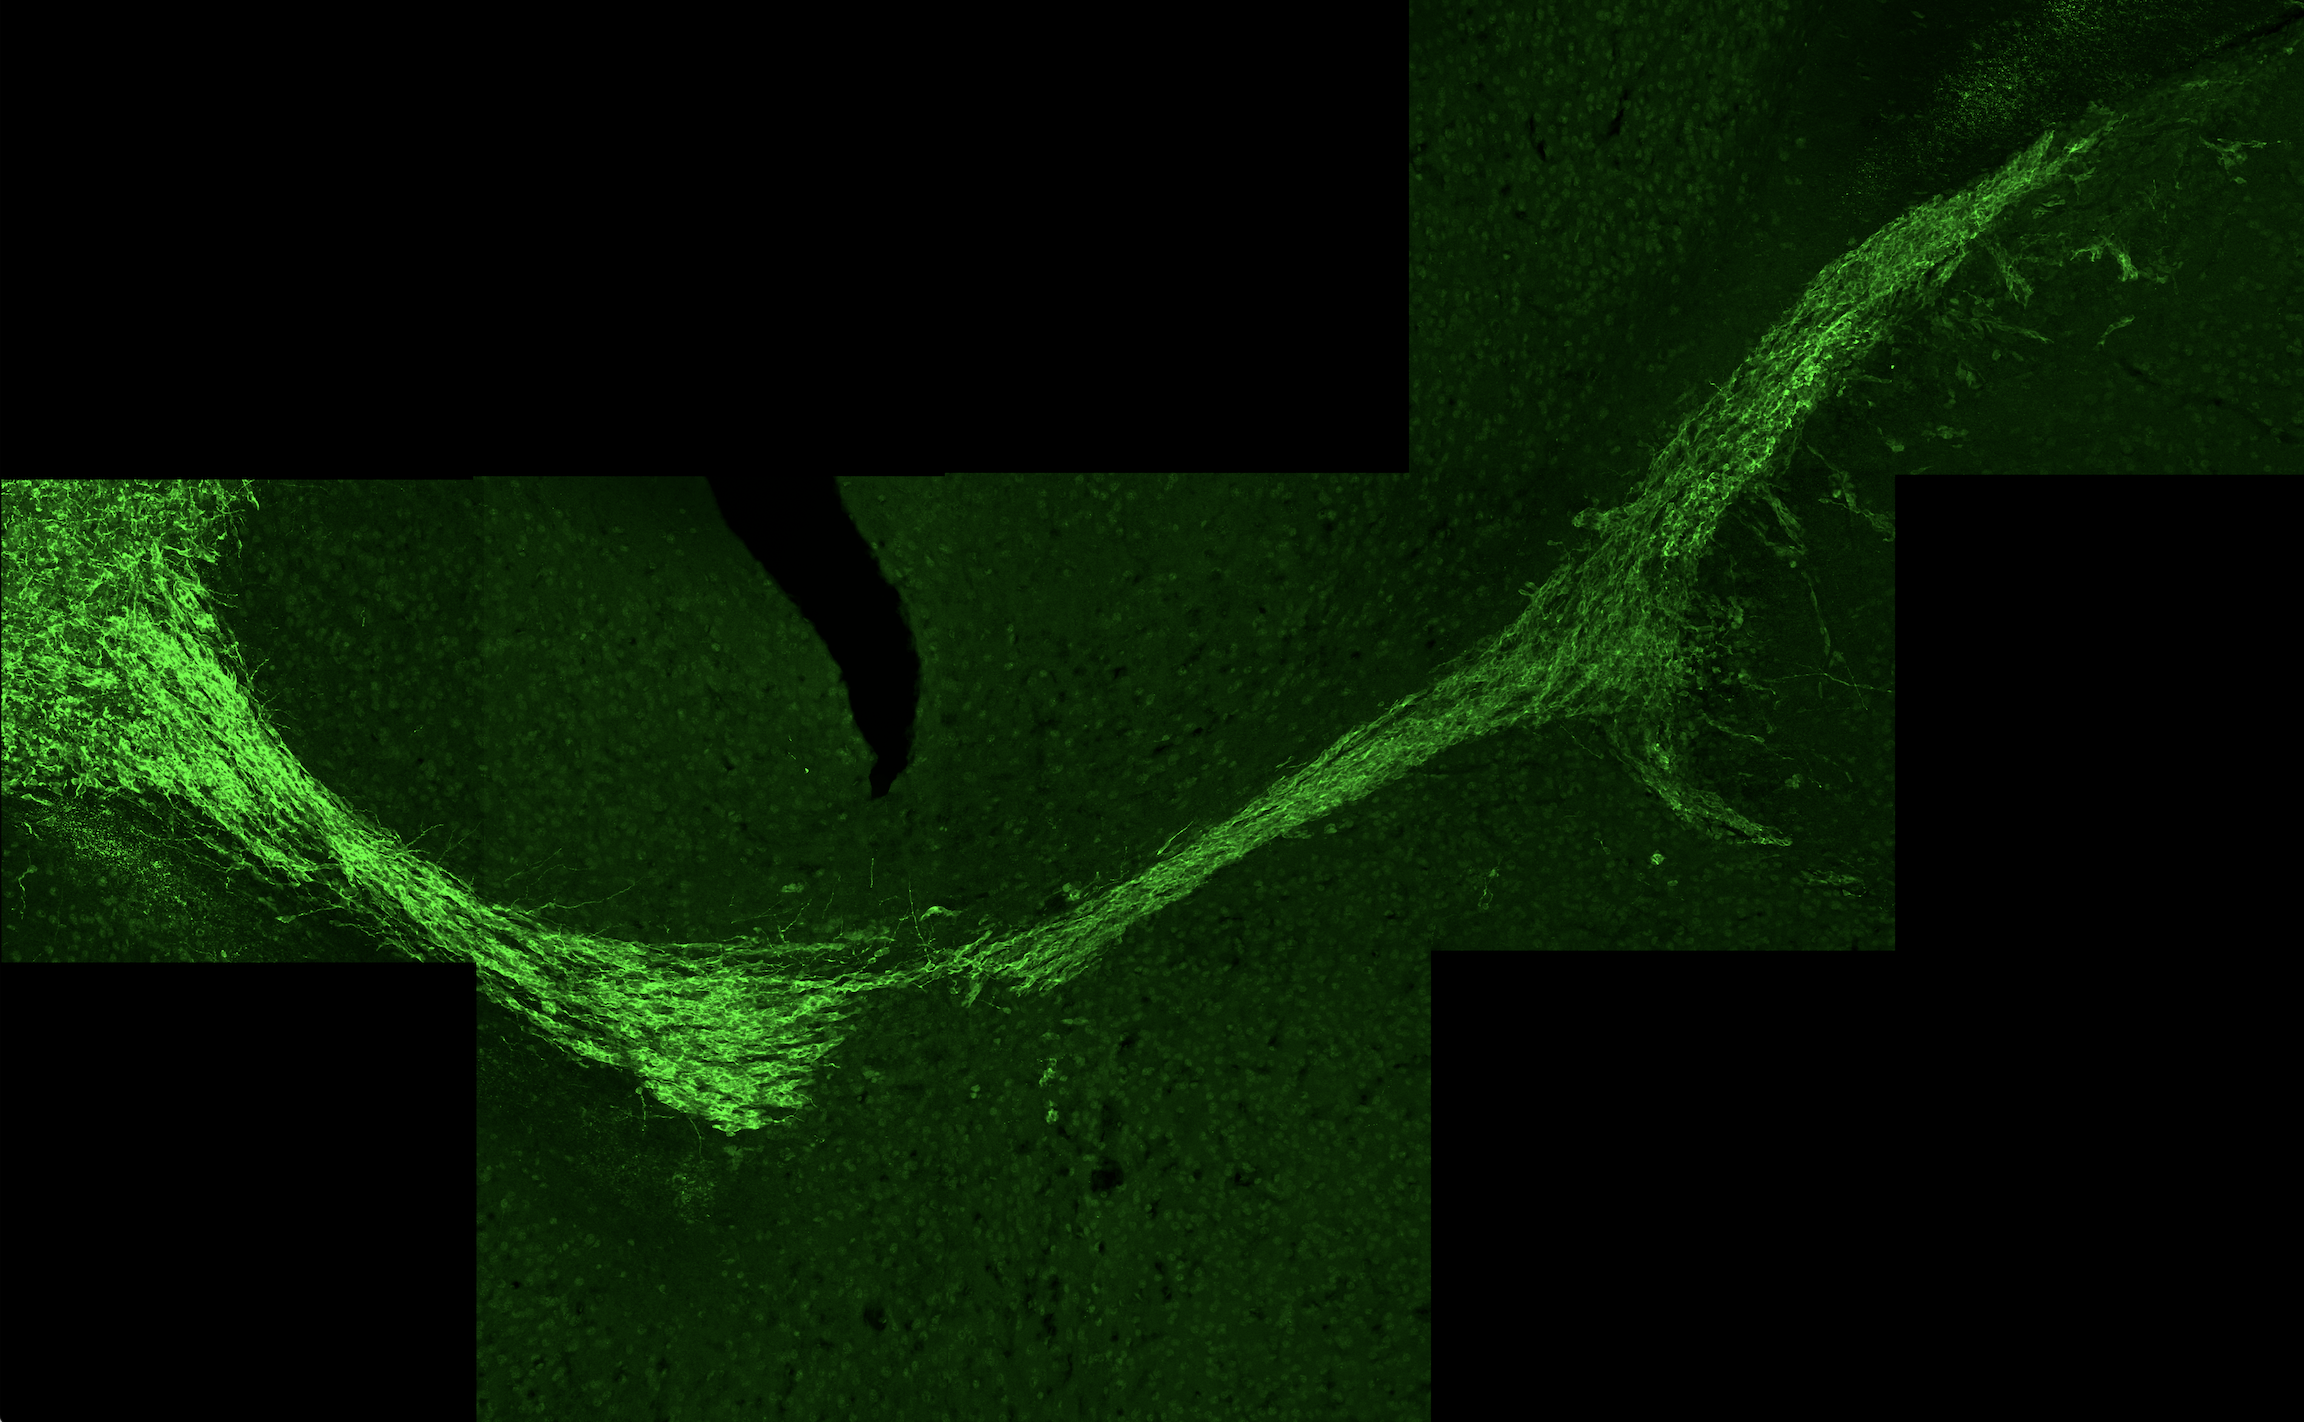
\includegraphics[width=0.95\linewidth]{via-verde}}
\end{frame}

\begin{frame}{Segundo objetivo: modelización y ajuste de parámetros}
	\begin{equation}
	\label{eq:neuroblast}
	\tau u_t + \X\, \nabla \cdot(u\nabla \O) + \alpha\, u - \gamma\, u \,1_{\NZdomain} 
	= \beta\, 1_{\SVZdomain}  
	\qquad\text{in}\enspace\Omega\times [0,T],
	\end{equation}
	\vspace{3mm}
	\begin{equation}
	\label{source}
	f_{\O}(x,y) = f_{\O}(\SO; x,y) 
	=  e^{((x-x_O)^2 + (y-y_O)^2)/\SO^2}.
	\end{equation}
	\vspace{3mm}
	\begin{equation} 
	\label{ob}
	\left\{ \begin{aligned} \Olf-\nabla\cdot (\mu_\CCdomain\,\nabla \Olf) &= f_{\O}  \quad  \text{ in } \Omega, \\
	\Olf &= f_{\O}  \quad \text{ on } \partial\Omega.
	\end{aligned}
	\right.
	\end{equation}
\end{frame}

\begin{frame}{Cerebro virtual}
	Malla
	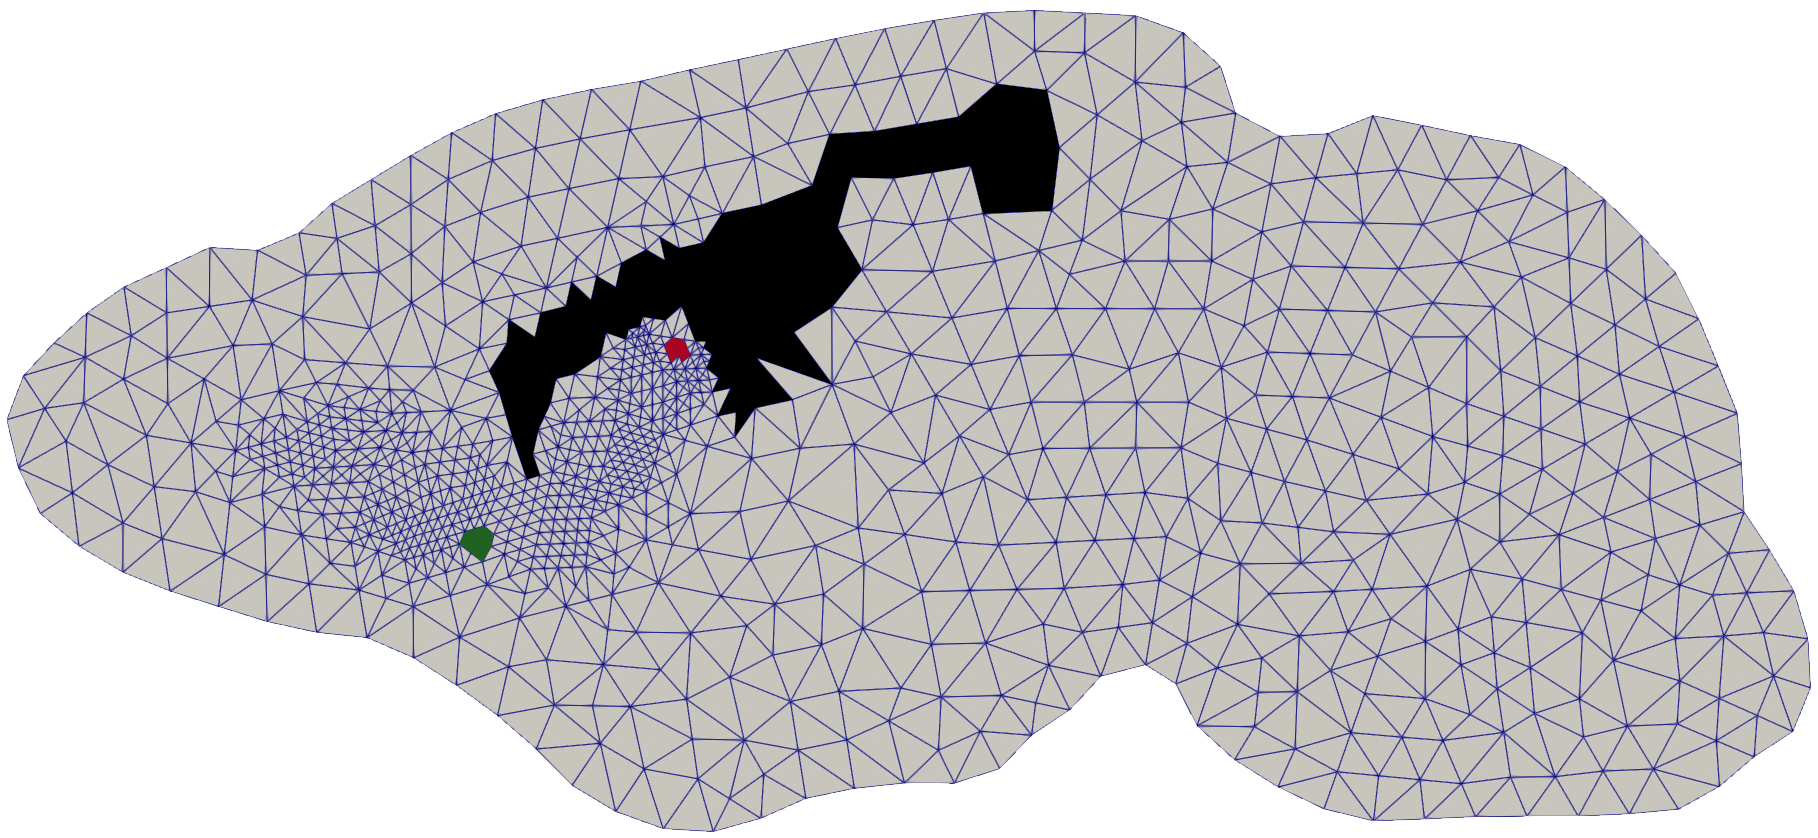
\includegraphics[width=0.95\linewidth]{brain-mesh.png}
\end{frame}

\begin{frame}{Modelización de la atracción}
Gradiente del bulbo olfatorio: parámetro $\sigma$
 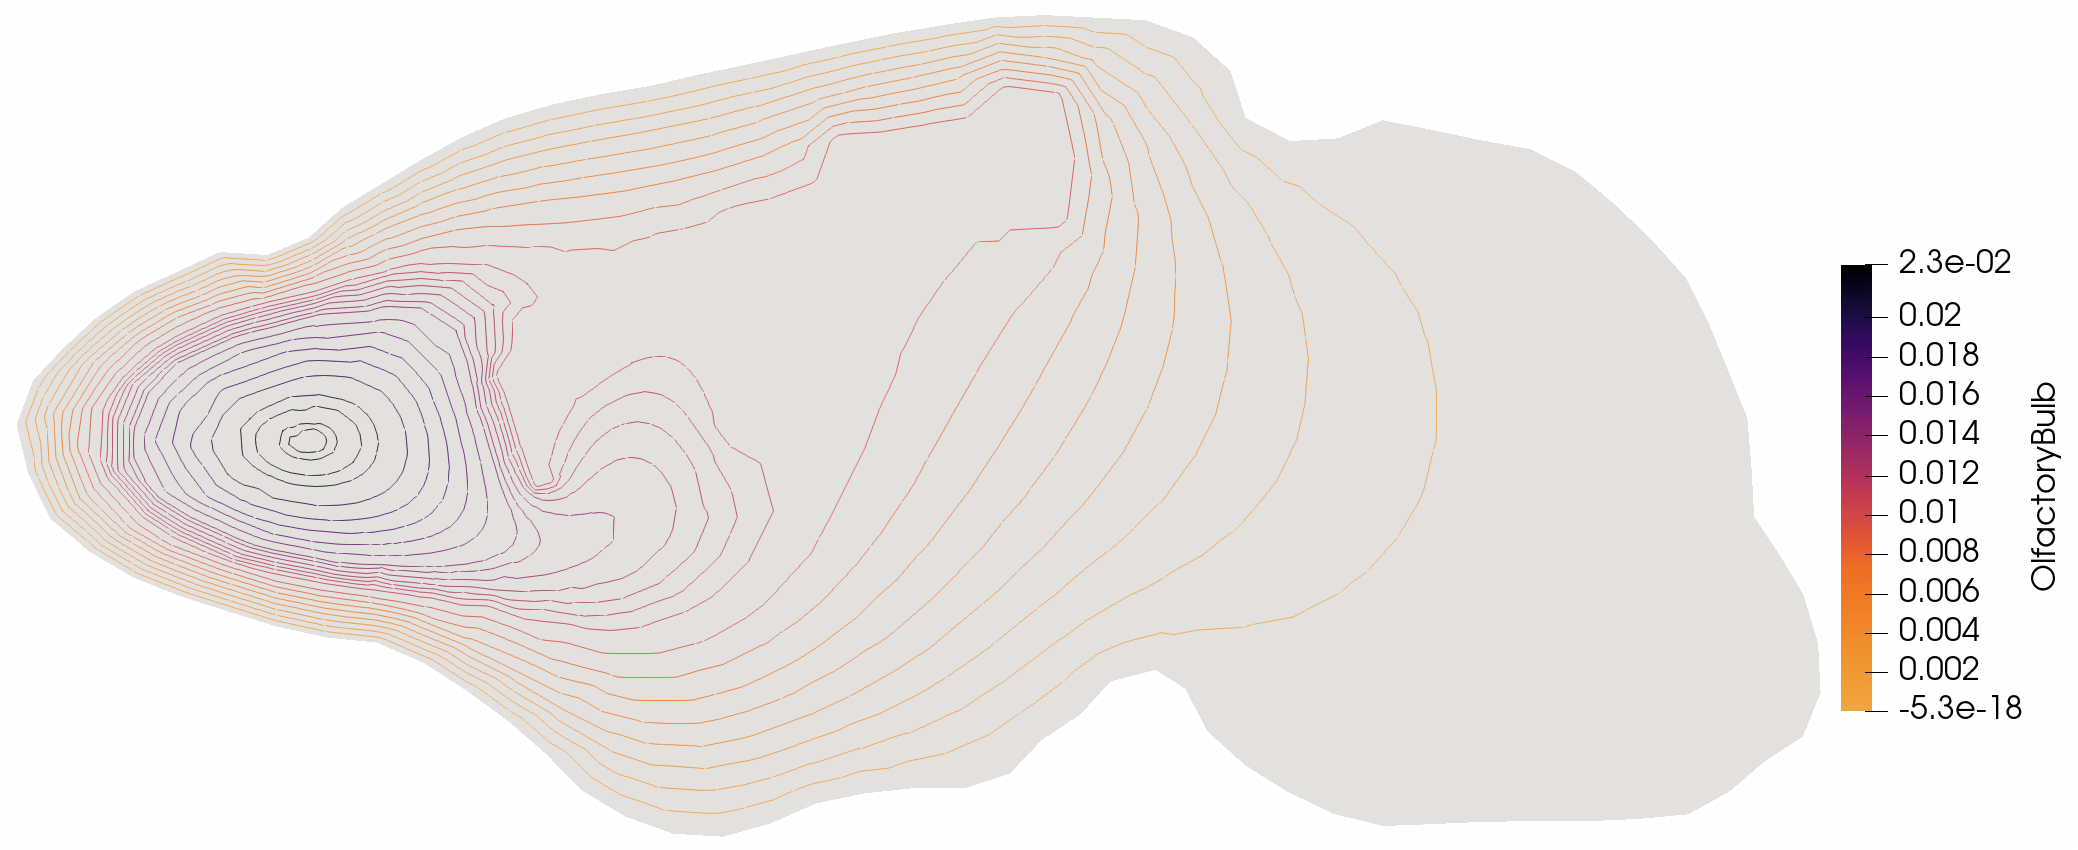
\includegraphics[width=0.95\linewidth]{ob.png}
\end{frame}
\begin{frame}{Modelización del movimiento}
	Vía rostral: parámetros $\alpha, \beta, \X, \gamma$
	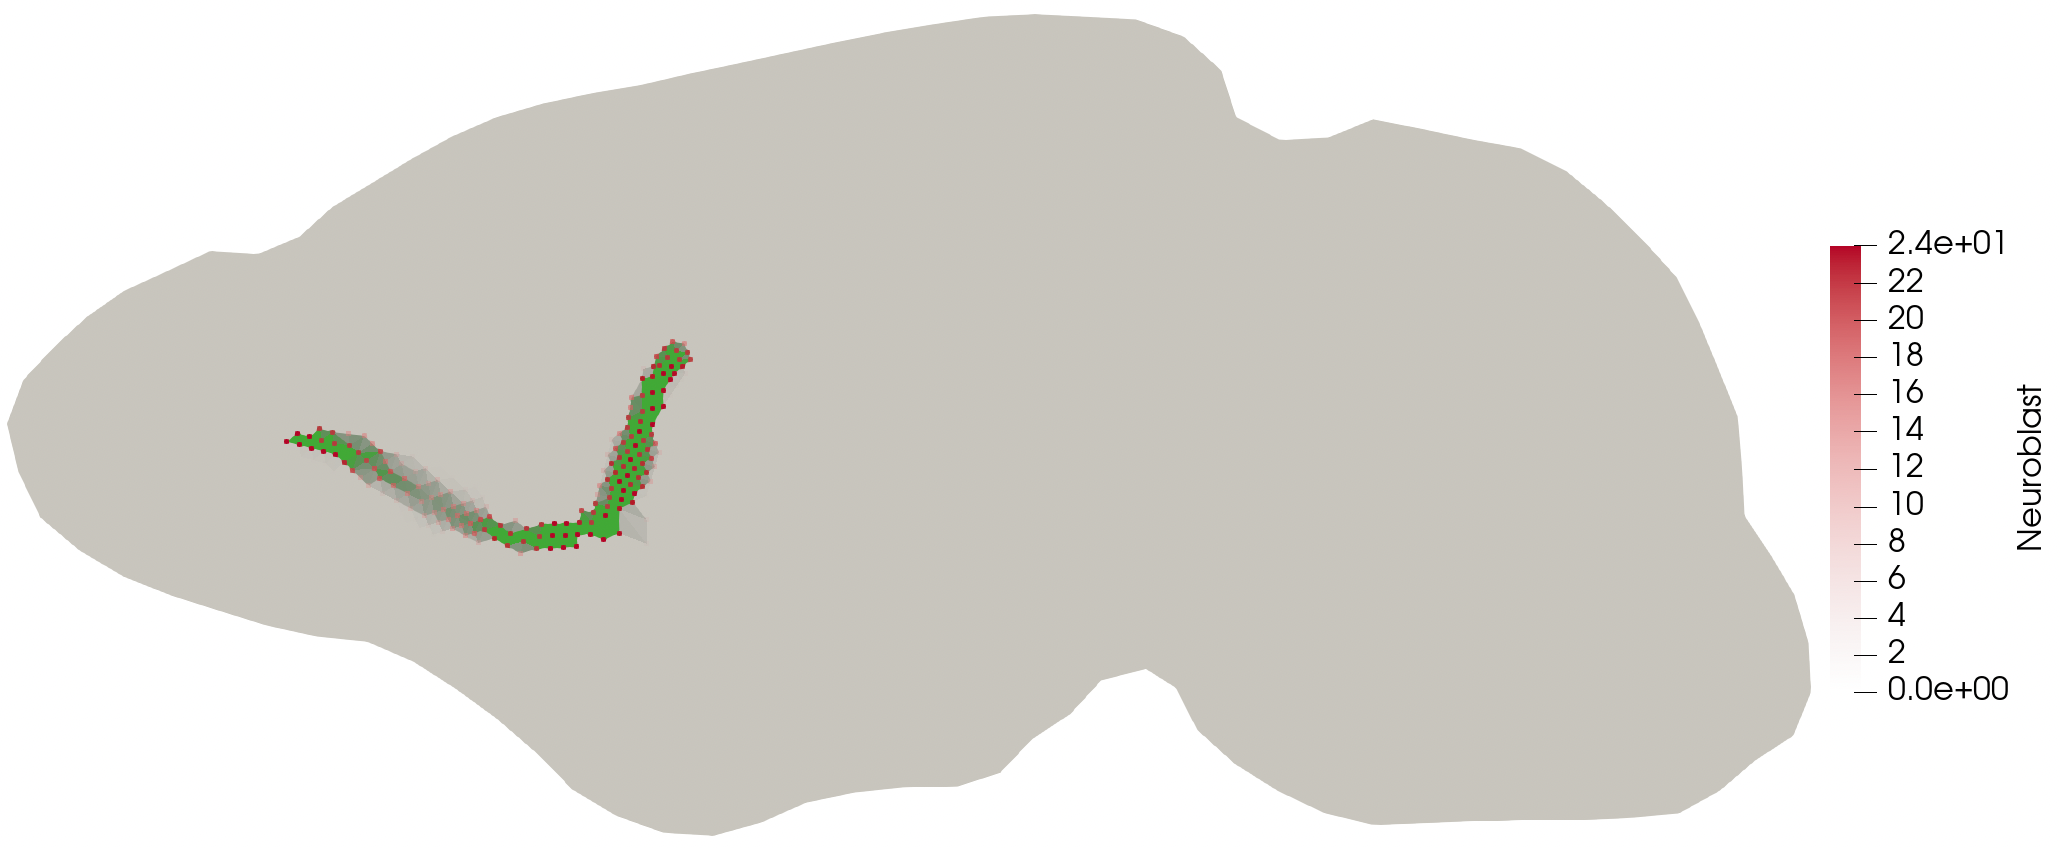
\includegraphics[width=0.95\linewidth]{steady-opt.png}
\end{frame}




%\include{dan1}
%
%% Beamer style >>>>>>>>>>>>>>>>>>>>>>>>>

\setbeamertemplate{enumerate item}[mycircle]

\setbeamertemplate{frametitle continuation}[from second][] % No automatic symbols I II II
%<<<<<<<<<<<<< beamer style

%\title{Redes Neuronales y otros Artefactos Matemáticos\vspace{-0.5em}}
%\author[J.R. Rodr\'{\i}guez Galv\'an]{\em\structure{Daniel Acosta Soba, Noelia Ortega Román, Álex Pérez Fernández, Rafa Rodríguez Galván}\vspace{-1.5em}}
%\date{\scriptsize{Facultad de Ciencias, Universidad de C\'adiz}\\[0.9em]\small Día Internacional de las Matemáticas («día {\Huge$\pi$}»), 2023}

% XeLaTeX font choosing
% \usepackage{fontspec}%{xltxtra} %fontspec}
% \setsansfont{Fontin Sans}
% \setsansfont{Lato}


\setcounter{tocdepth}{1}
\newcommand{\Olf}{\mathcal{O}}
\newcommand{\SVZdomain}{\text{\it SVZ}}
\newcommand{\NZdomain}{\text{\it NZ}}
\newcommand{\CCdomain}{{\text{\it CC}}}
\newcommand{\CCexp}{\mu_{CC}}
\newcommand{\tCCexp}{\tilde{\mu}_{CC}}
\def\SO{\sigma}
\def\X{\chi}
\def\D{\mathscr{D}}
\def\T{\mathcal{T}}
\def\E{\mathcal{E}}
\def\S{\mathcal{S}}
\def\N{\mathbb{N}}
\def\P{\mathbb{P}}
\def\O{\mathcal{O}}

%
% Bibliography
%
%\usepackage{natbib}

% To list each bibliographic entry in a line
\setbeamertemplate{bibliography entry title}{}
\setbeamertemplate{bibliography entry location}{}
\setbeamertemplate{bibliography entry note}{}

% ... end of preamble.

\AtBeginSection{\frame{\sectionpage}}

\colorlet{inputcolor}{green!60!black}
\colorlet{hiddencolor}{blue!60!black}
\colorlet{outcolor}{red!60!black}

%======================================================================

%======================================================================

% Tikz style and beamer template ------->>>
\tikzstyle{every picture}+=[remember picture]
\tikzstyle{na} = [baseline=-.5ex]
\tikzstyle{phd} = [baseline=-.6ex,
  box/.style={rectangle, draw=PHDblueC, thick, fill=PHDblueA,
    align=center, rounded corners, minimum height=1.6em},
  boxB/.style={rectangle, draw=PHDredA, thick, fill=PHDblueA,
    align=center, rounded corners, minimum height=1.6em}]
\tikzstyle{phdB} = [baseline=-.7ex,
  box/.style={rectangle, draw=PHDblueC, thick, fill=PHDblueA,
    align=center, rounded corners, minimum height=1.6em},
  boxB/.style={rectangle, draw=PHDredA, thick, fill=PHDblueA,
    align=center, rounded corners, minimum height=1.6em}]
\tikzstyle{myarrow} = [->,>=latex, PHDredA, shorten >=4pt,
  opacity=.6, line width=0.6mm]
\tikzstyle{myarrow2} = [->,>=latex, PHDblueC, shorten >=4pt, opacity=.2, line width=0.4mm]
\tikzstyle{myarrow3} = [
     opacity=.7,
%    >=triangle 60,              % Nice arrows; your taste may be different
    node distance=6mm and 60mm, % Global setup of box spacing
    every join/.style={norm},   % Default linetype for connecting
                                % boxes
    line width=0.6mm,
    PHDredA,
    ->
    ]
\setbeamertemplate{background}
 {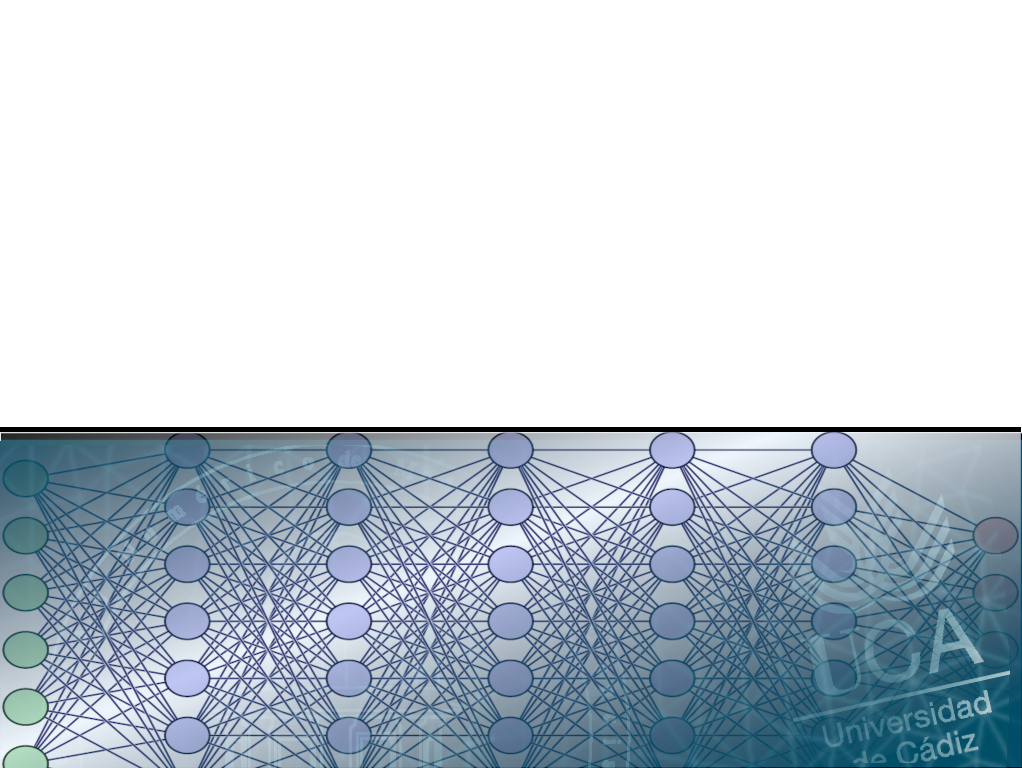
\includegraphics[width=\paperwidth,height=\paperheight]{frontpage_bg}}
\setbeamertemplate{footline}[default]
% <<<-------


% Write custom titlepage ------->>>
%\begin{frame}
%  \titlepage
%  \vspace{5cm}
%\end{frame}

% Set the background for the rest of the slides.
\setbeamertemplate{background}{}
 % {
\includegraphics[width=\paperwidth,height=\paperheight]{slide_bg}}


% Write all of the slides..........

% \begin{frame}{Outline}
%   \tableofcontents
% \end{frame}

% Start inserting infoline at the end
\setbeamertemplate{footline}[PHDtheme]
% <<<-------

%\newcommand{\imgdir}{Undefined, use renewcommand!}

%============================================================================
\section{Migración de neuroblastos en el cerebro adulto}
%============================================================================

%=====================================================================
\begin{frame}{¿Qué queremos modelar?}
%---------------------------------------------------------------------
\only<1>{
  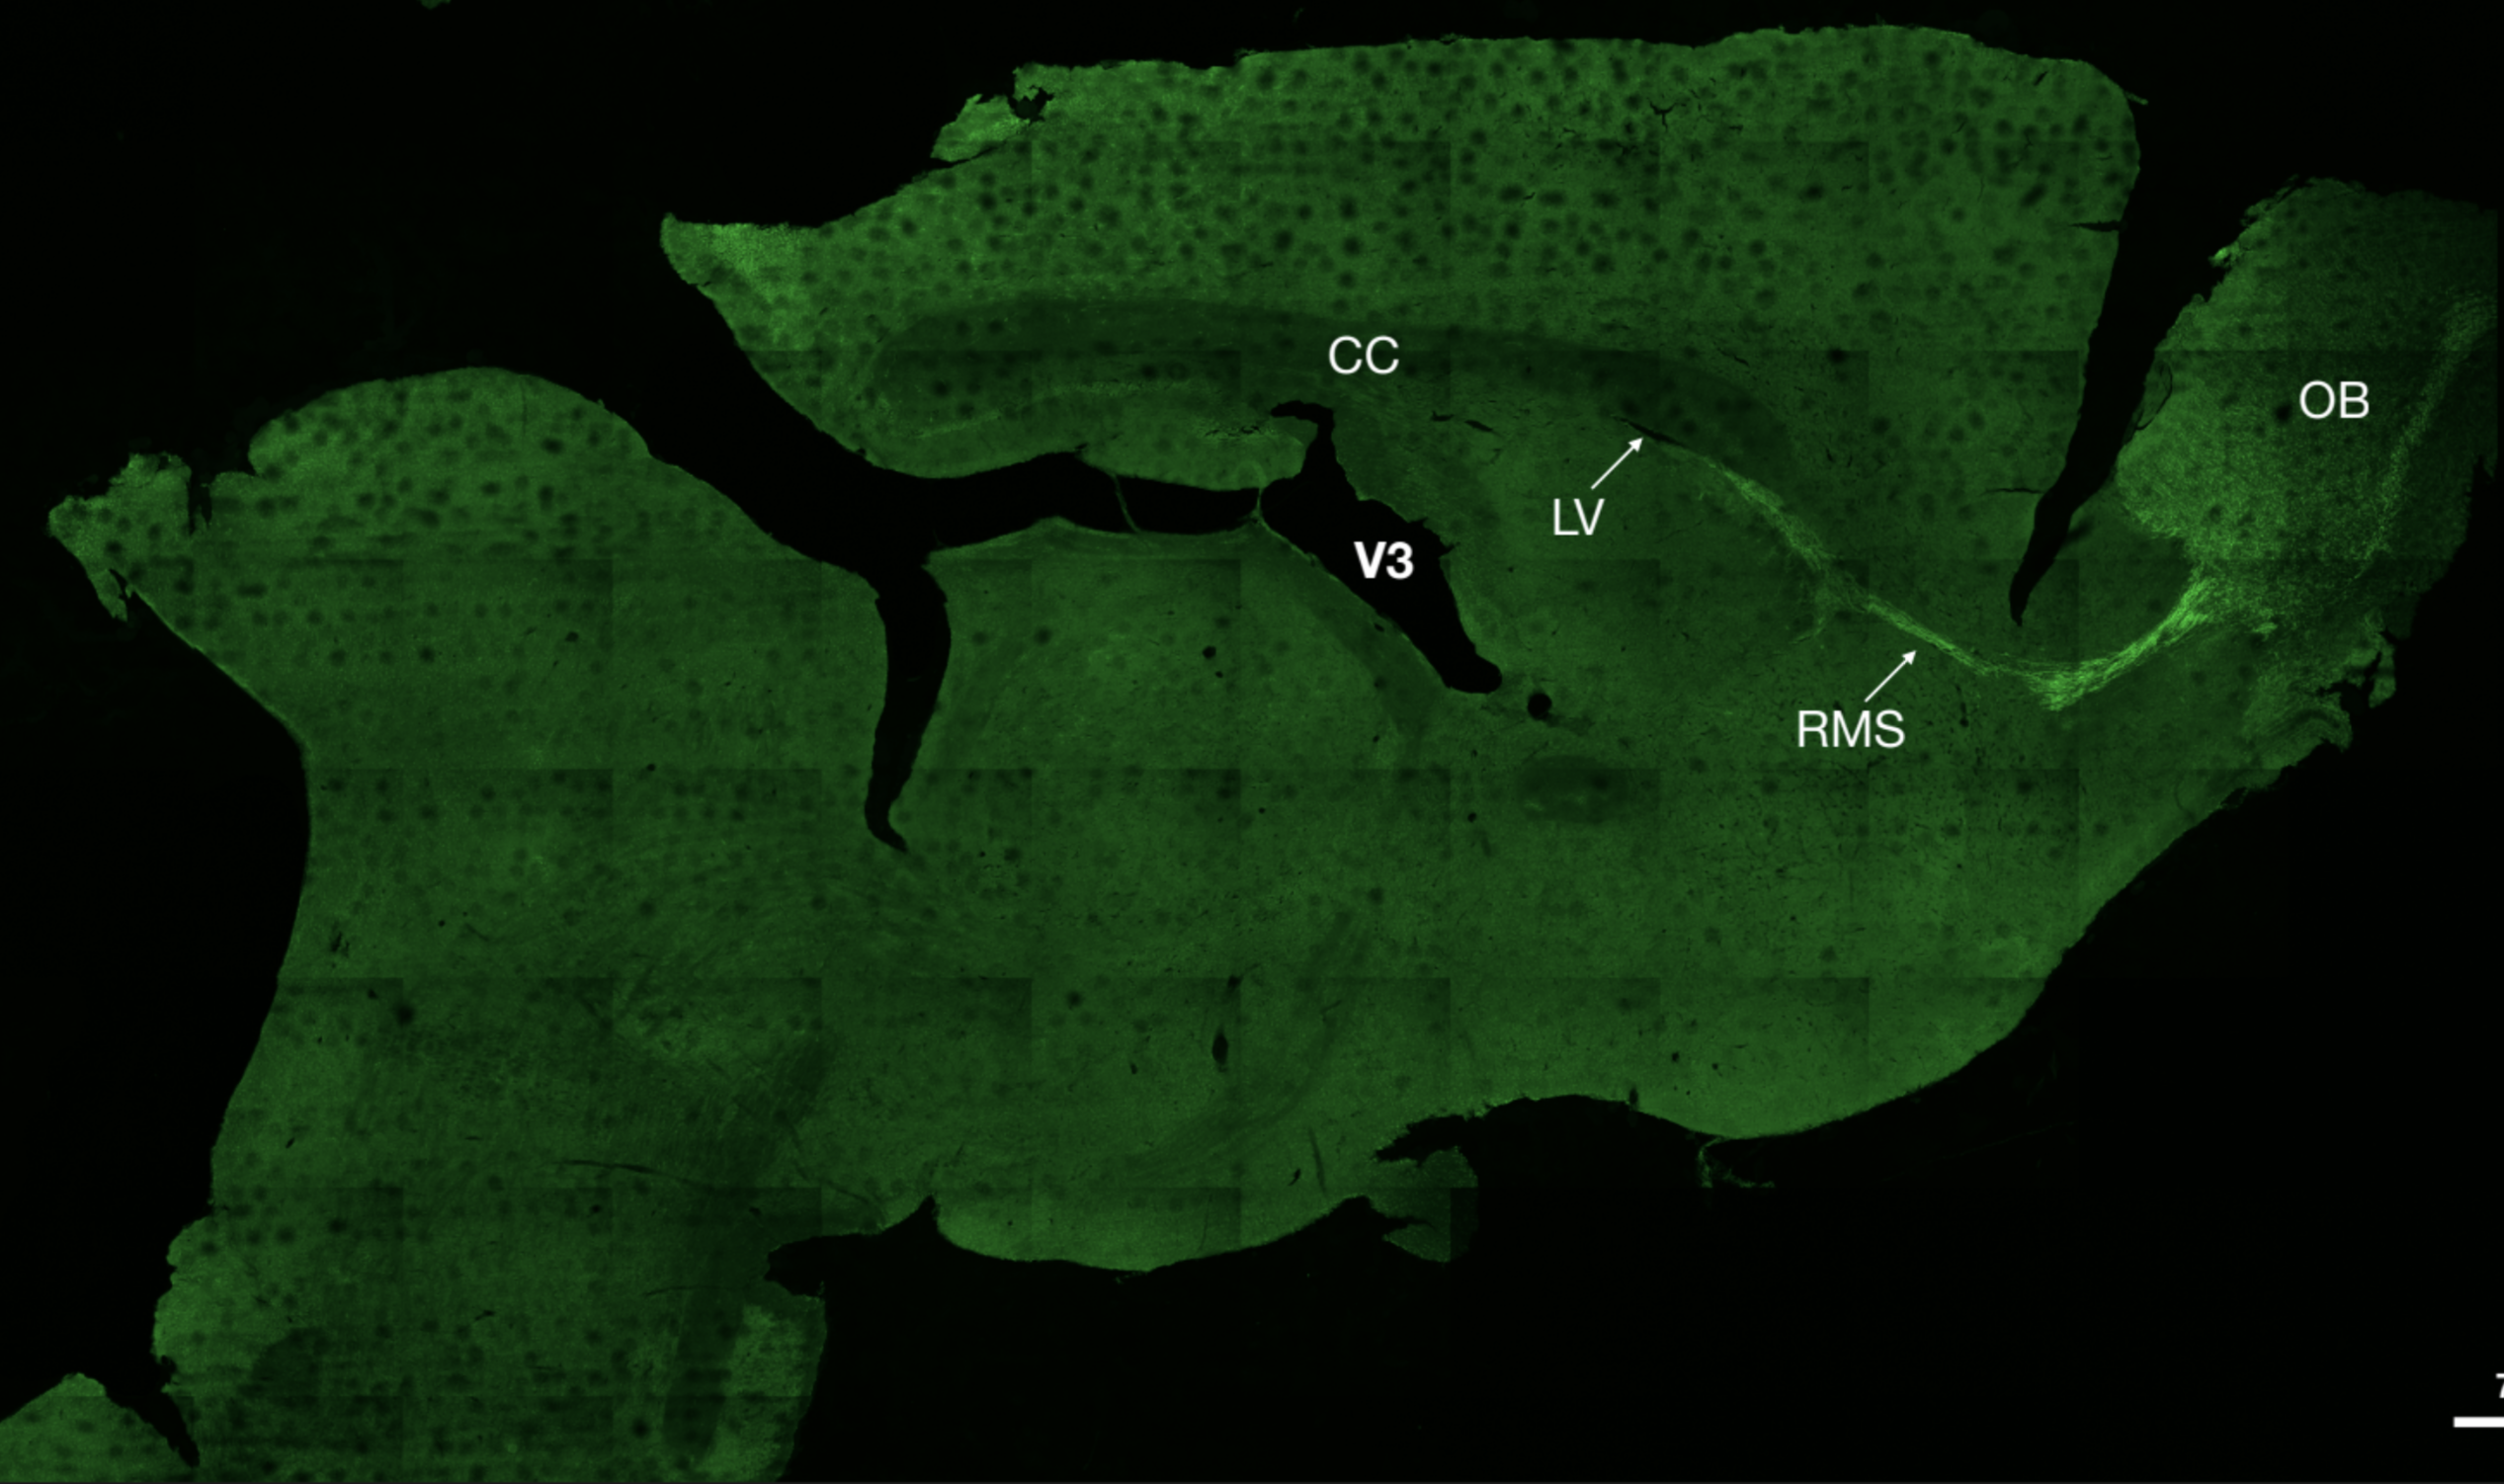
\includegraphics[width=0.95\linewidth]{cerebro-completo}}
  \only<2->{
  \includegraphics[width=0.95\linewidth]{via-rostral}}
\end{frame}

\begin{frame}{Primer objetivo: recuento de neuroblastos}
  \only<1>{
  	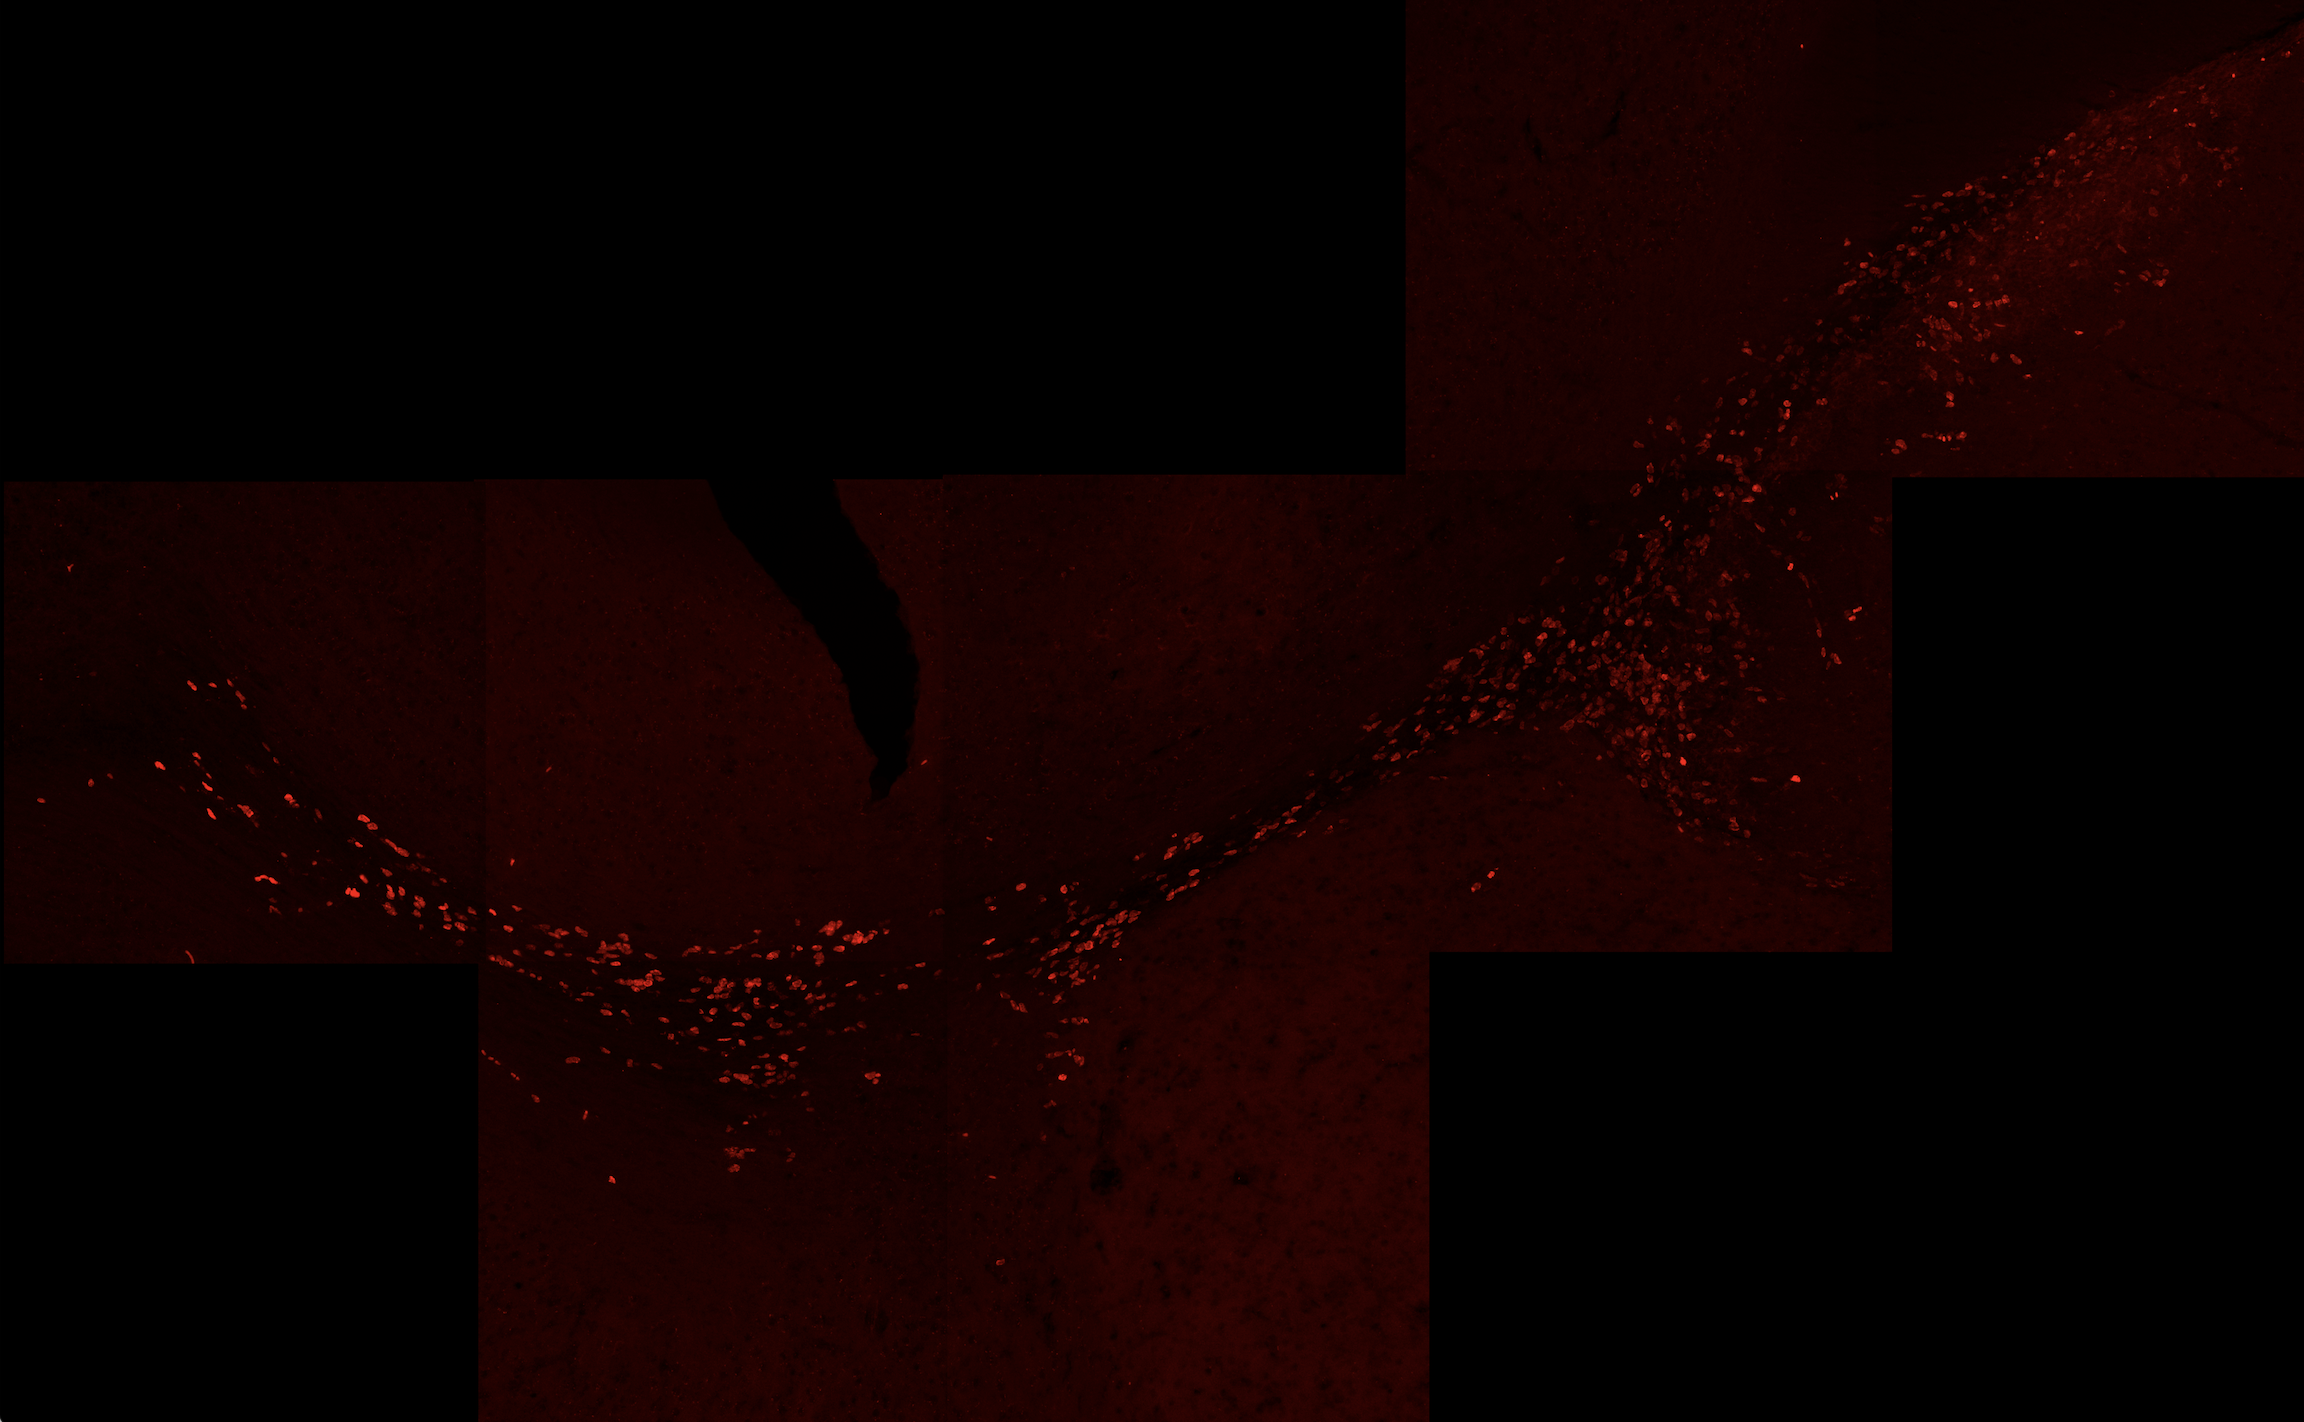
\includegraphics[width=0.95\linewidth]{via-roja}}
  \only<2->{
  	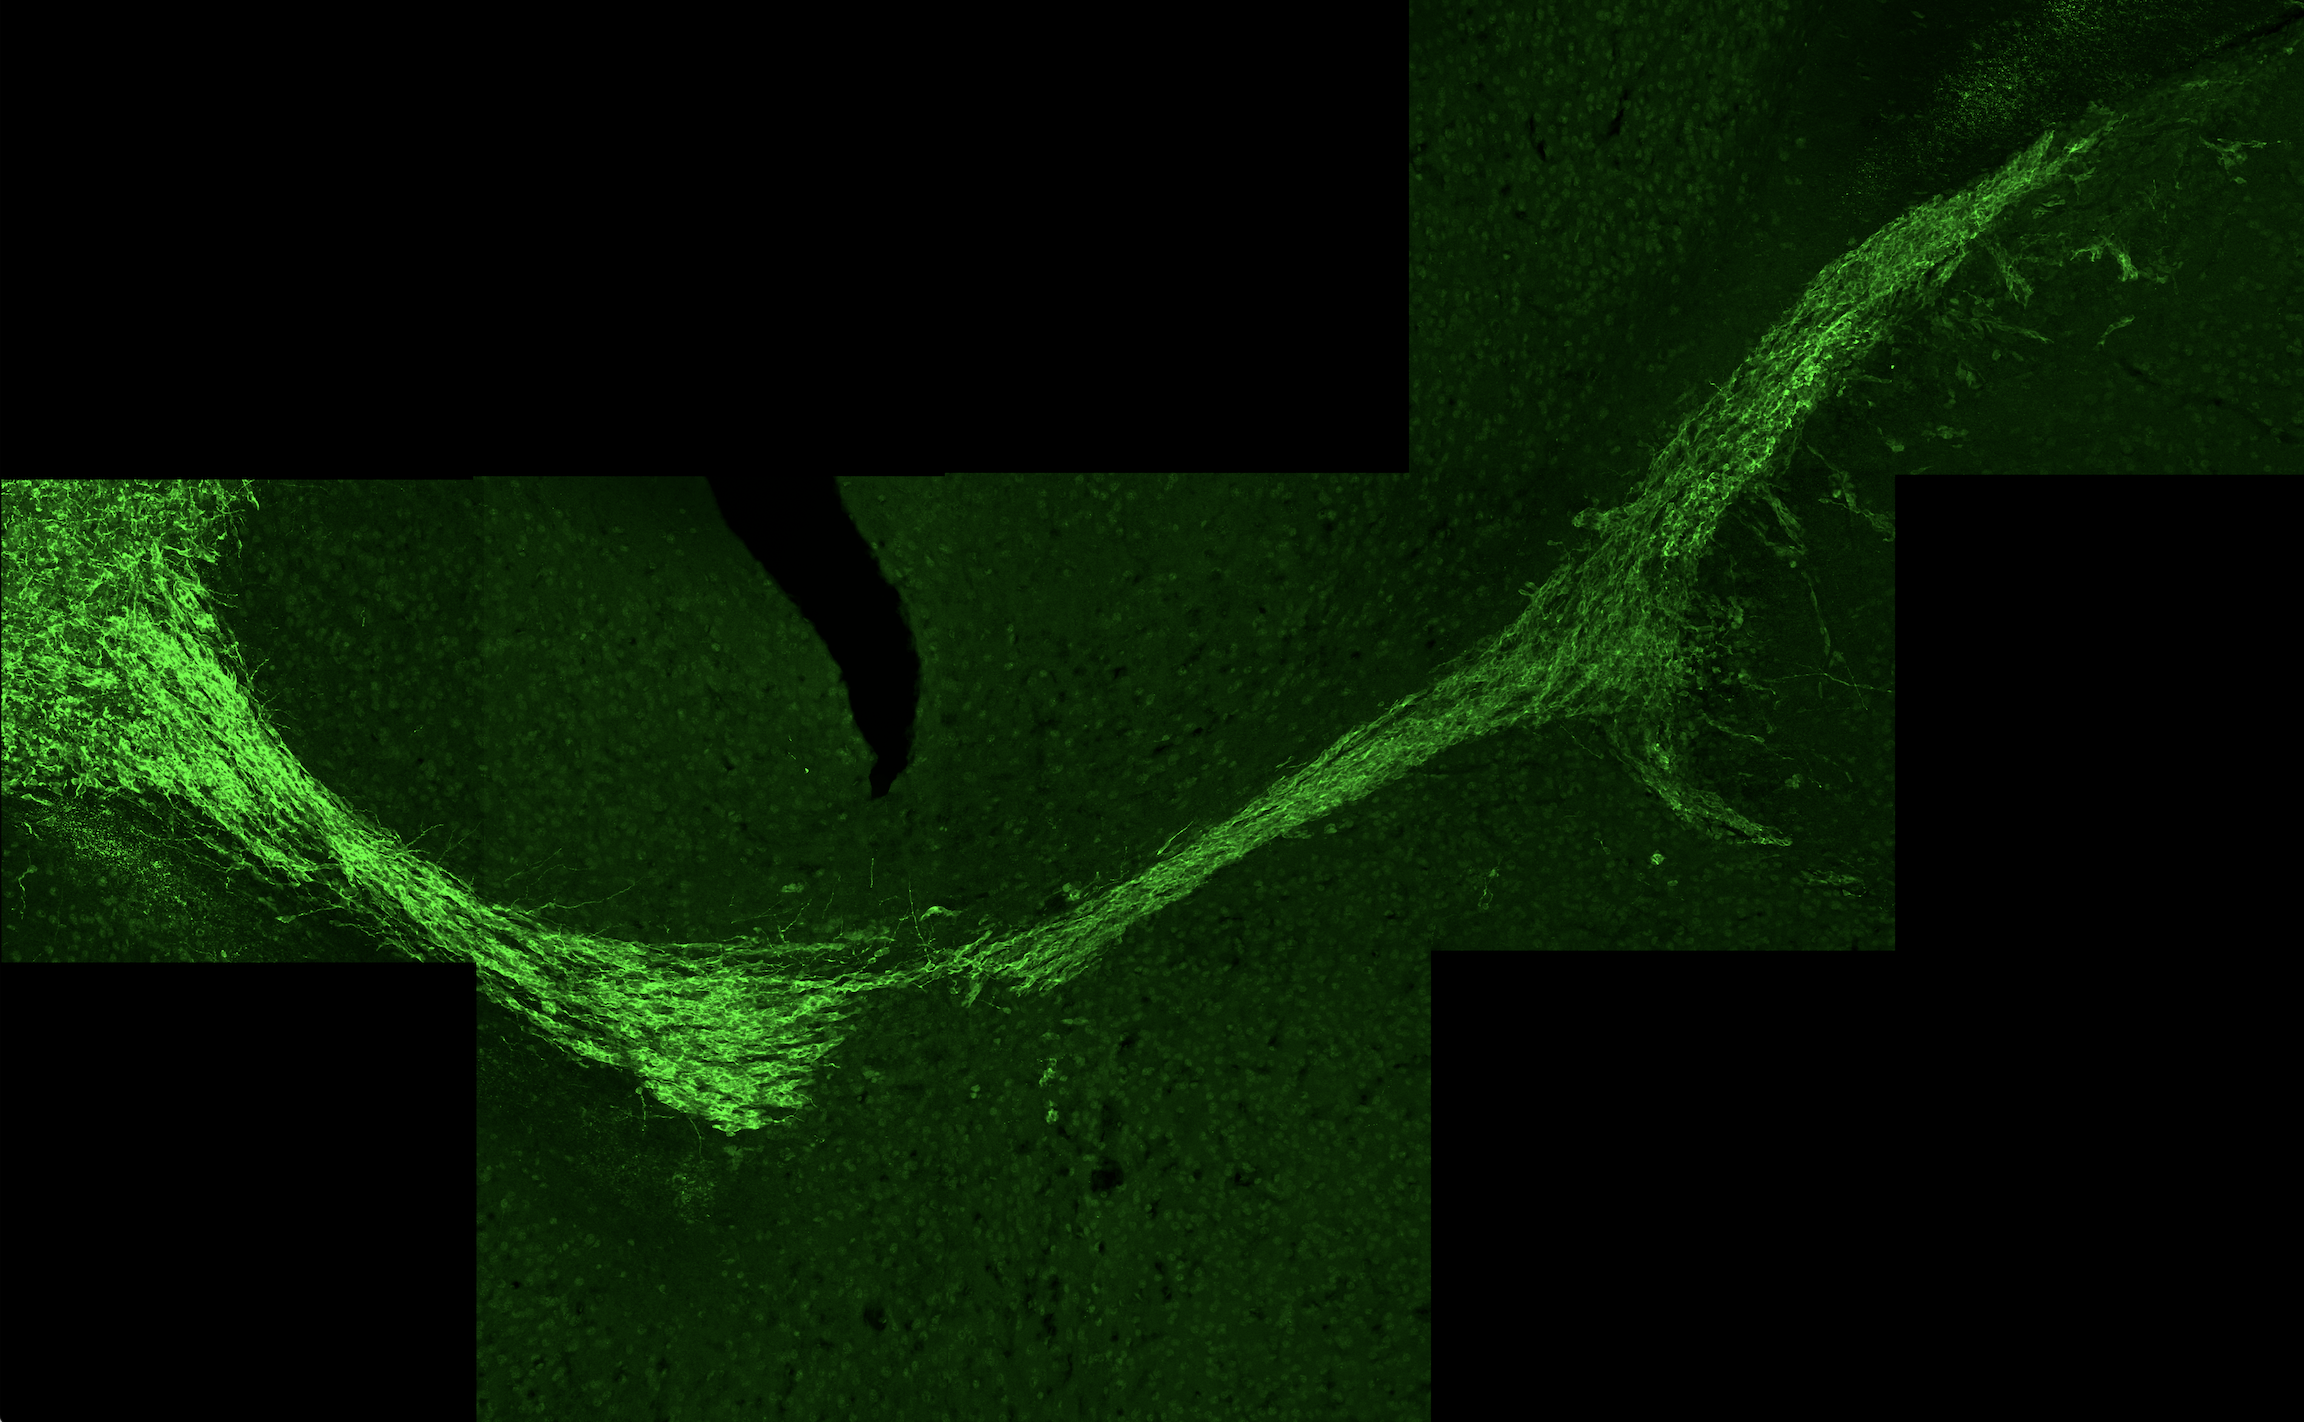
\includegraphics[width=0.95\linewidth]{via-verde}}
\end{frame}

\begin{frame}{Segundo objetivo: modelización y ajuste de parámetros}
	\begin{equation}
	\label{eq:neuroblast}
	\tau u_t + \X\, \nabla \cdot(u\nabla \O) + \alpha\, u - \gamma\, u \,1_{\NZdomain} 
	= \beta\, 1_{\SVZdomain}  
	\qquad\text{in}\enspace\Omega\times [0,T],
	\end{equation}
	\vspace{3mm}
	\begin{equation}
	\label{source}
	f_{\O}(x,y) = f_{\O}(\SO; x,y) 
	=  e^{((x-x_O)^2 + (y-y_O)^2)/\SO^2}.
	\end{equation}
	\vspace{3mm}
	\begin{equation} 
	\label{ob}
	\left\{ \begin{aligned} \Olf-\nabla\cdot (\mu_\CCdomain\,\nabla \Olf) &= f_{\O}  \quad  \text{ in } \Omega, \\
	\Olf &= f_{\O}  \quad \text{ on } \partial\Omega.
	\end{aligned}
	\right.
	\end{equation}
\end{frame}

\begin{frame}{Cerebro virtual}
	Malla
	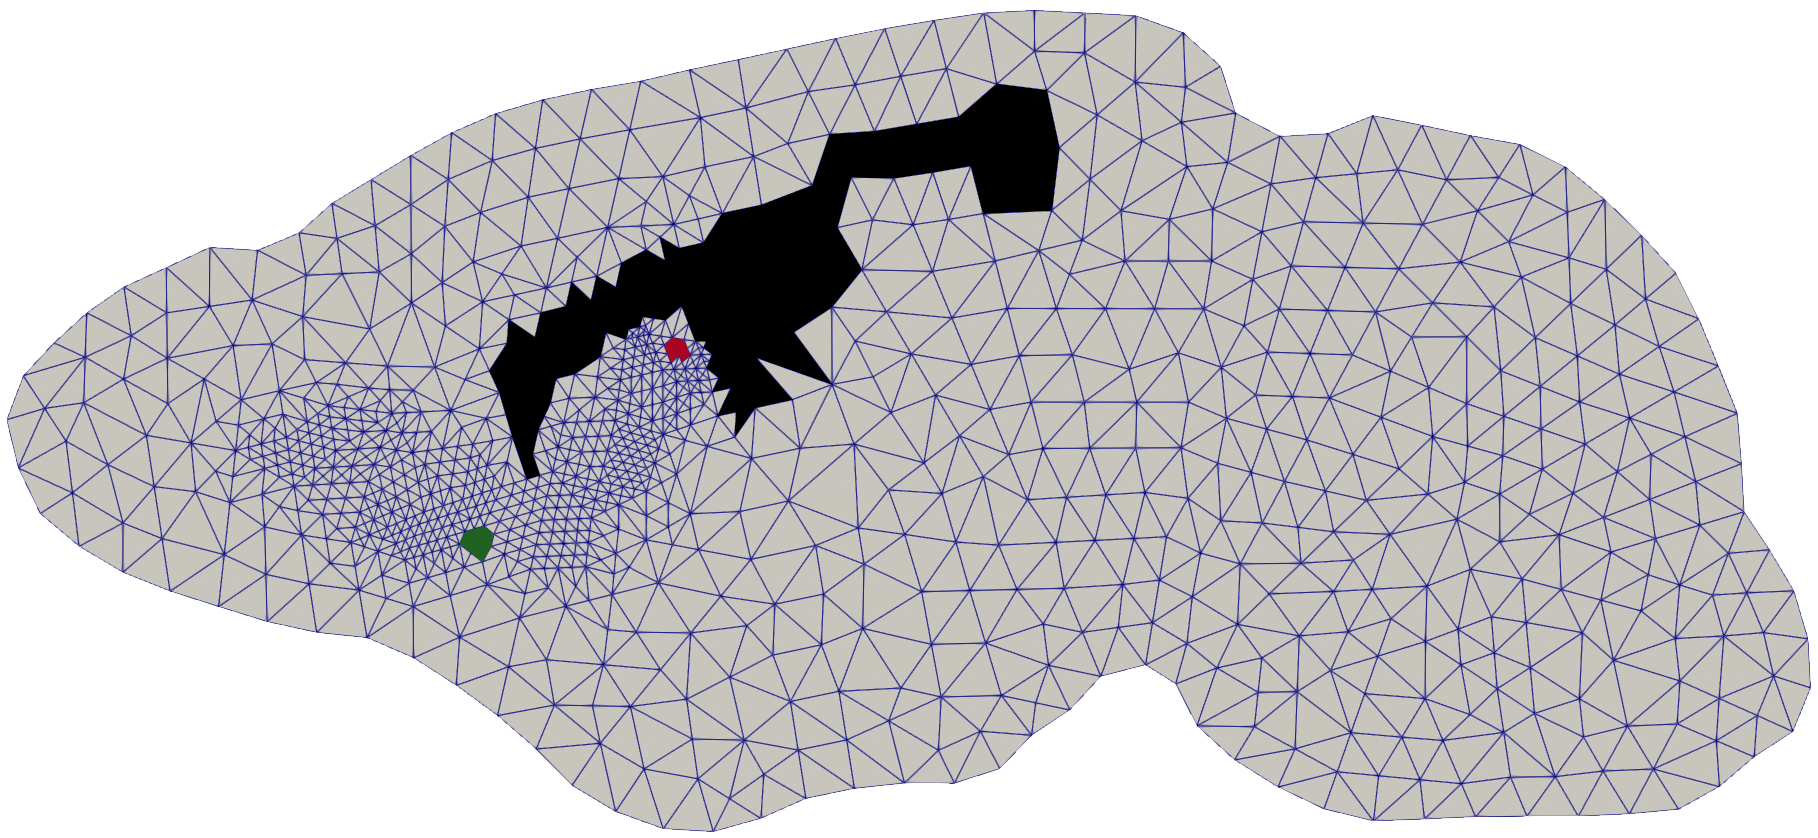
\includegraphics[width=0.95\linewidth]{brain-mesh.png}
\end{frame}

\begin{frame}{Modelización de la atracción}
Gradiente del bulbo olfatorio: parámetro $\sigma$
 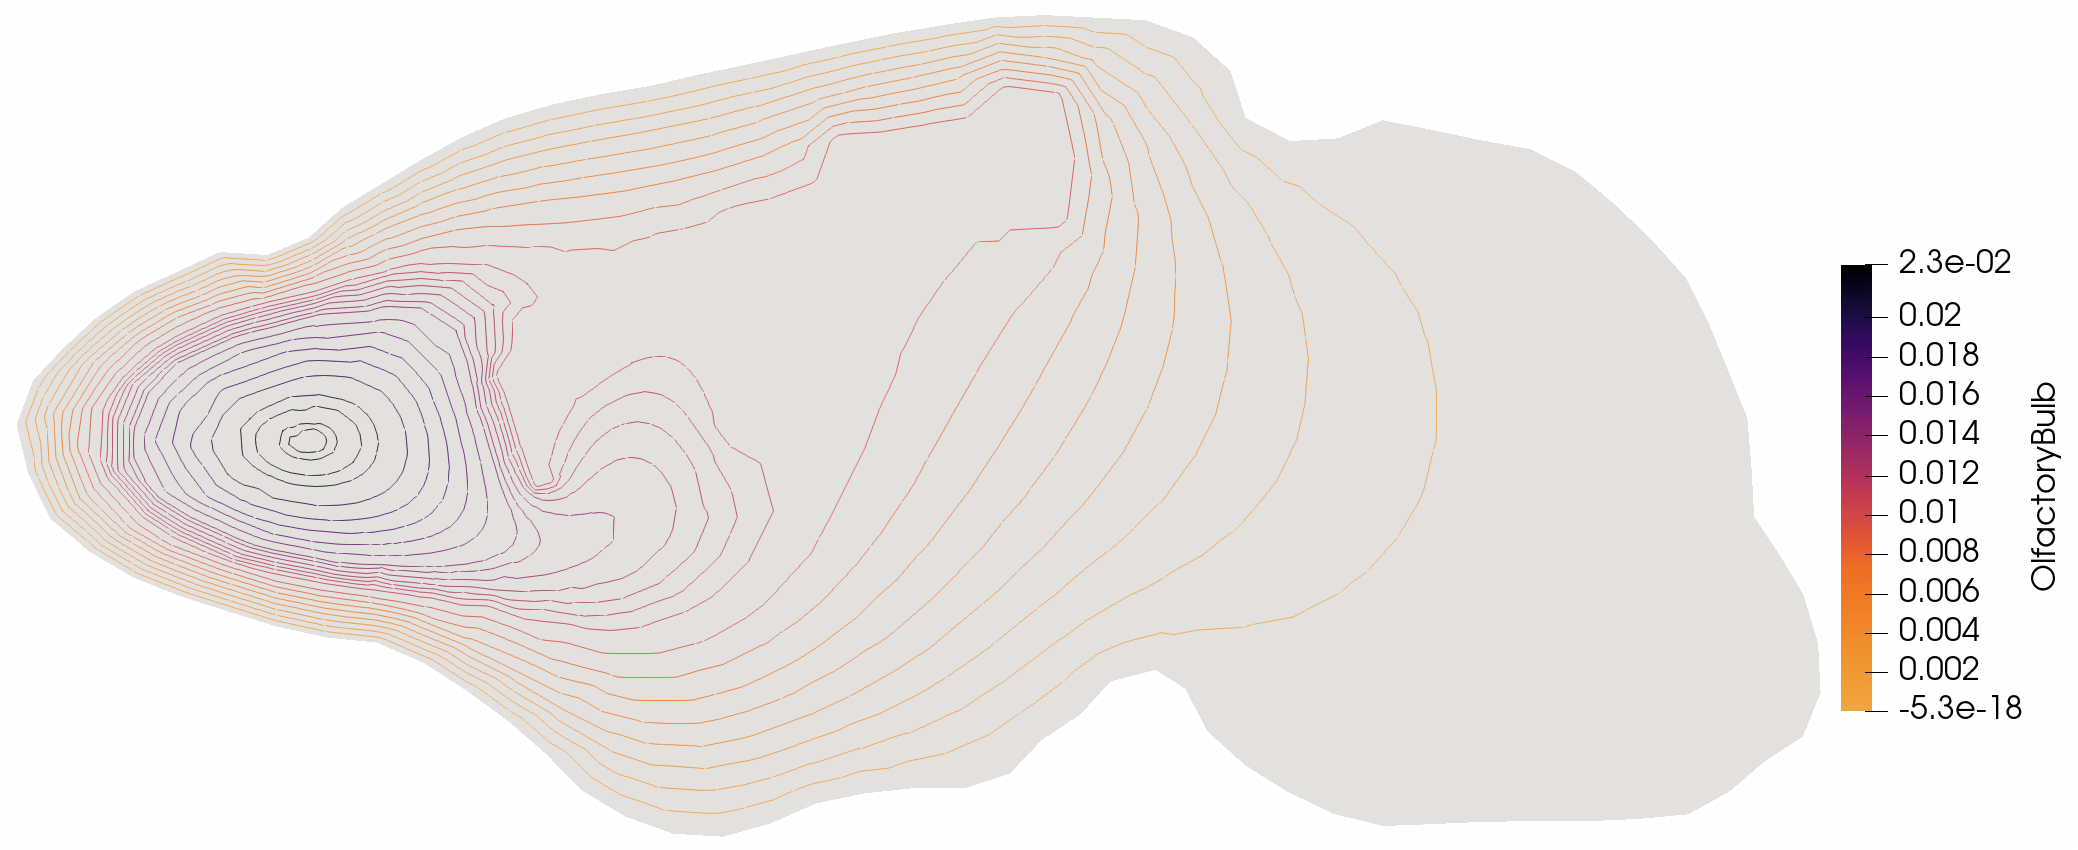
\includegraphics[width=0.95\linewidth]{ob.png}
\end{frame}
\begin{frame}{Modelización del movimiento}
	Vía rostral: parámetros $\alpha, \beta, \X, \gamma$
	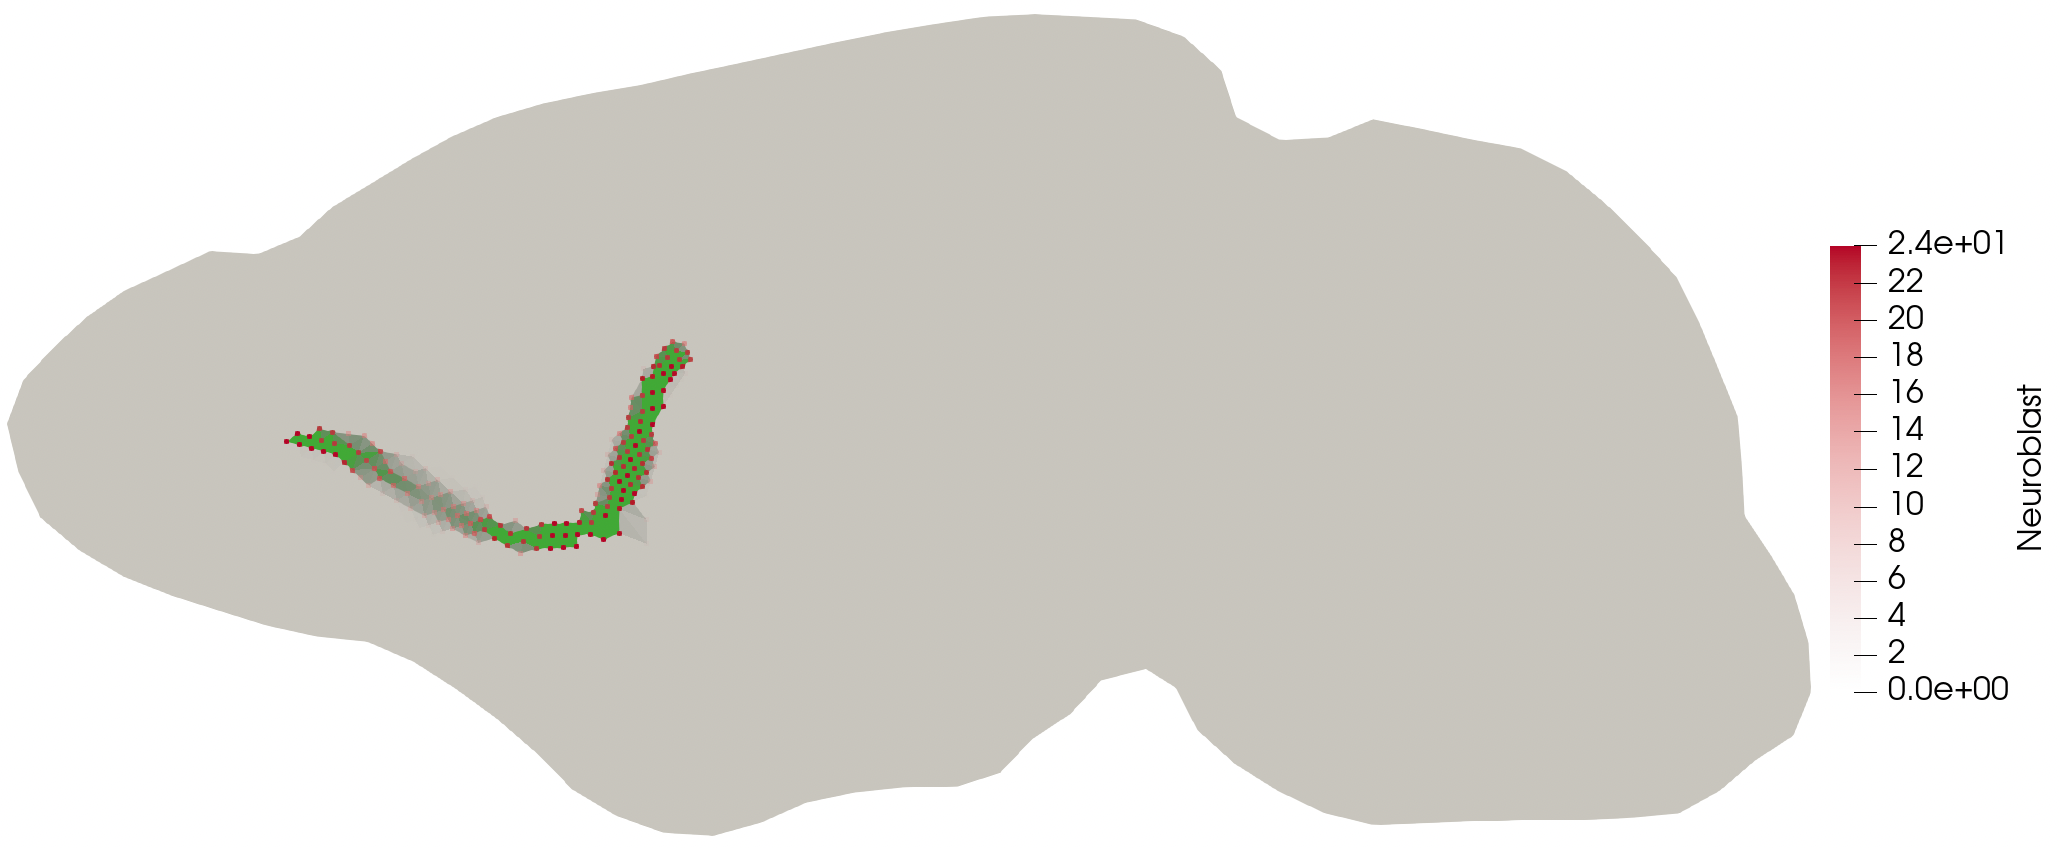
\includegraphics[width=0.95\linewidth]{steady-opt.png}
\end{frame}




%\include{dan1}
%
%% Beamer style >>>>>>>>>>>>>>>>>>>>>>>>>

\setbeamertemplate{enumerate item}[mycircle]

\setbeamertemplate{frametitle continuation}[from second][] % No automatic symbols I II II
%<<<<<<<<<<<<< beamer style

%\title{Redes Neuronales y otros Artefactos Matemáticos\vspace{-0.5em}}
%\author[J.R. Rodr\'{\i}guez Galv\'an]{\em\structure{Daniel Acosta Soba, Noelia Ortega Román, Álex Pérez Fernández, Rafa Rodríguez Galván}\vspace{-1.5em}}
%\date{\scriptsize{Facultad de Ciencias, Universidad de C\'adiz}\\[0.9em]\small Día Internacional de las Matemáticas («día {\Huge$\pi$}»), 2023}

% XeLaTeX font choosing
% \usepackage{fontspec}%{xltxtra} %fontspec}
% \setsansfont{Fontin Sans}
% \setsansfont{Lato}


\setcounter{tocdepth}{1}
\newcommand{\Olf}{\mathcal{O}}
\newcommand{\SVZdomain}{\text{\it SVZ}}
\newcommand{\NZdomain}{\text{\it NZ}}
\newcommand{\CCdomain}{{\text{\it CC}}}
\newcommand{\CCexp}{\mu_{CC}}
\newcommand{\tCCexp}{\tilde{\mu}_{CC}}
\def\SO{\sigma}
\def\X{\chi}
\def\D{\mathscr{D}}
\def\T{\mathcal{T}}
\def\E{\mathcal{E}}
\def\S{\mathcal{S}}
\def\N{\mathbb{N}}
\def\P{\mathbb{P}}
\def\O{\mathcal{O}}

%
% Bibliography
%
%\usepackage{natbib}

% To list each bibliographic entry in a line
\setbeamertemplate{bibliography entry title}{}
\setbeamertemplate{bibliography entry location}{}
\setbeamertemplate{bibliography entry note}{}

% ... end of preamble.

\AtBeginSection{\frame{\sectionpage}}

\colorlet{inputcolor}{green!60!black}
\colorlet{hiddencolor}{blue!60!black}
\colorlet{outcolor}{red!60!black}

%======================================================================

%======================================================================

% Tikz style and beamer template ------->>>
\tikzstyle{every picture}+=[remember picture]
\tikzstyle{na} = [baseline=-.5ex]
\tikzstyle{phd} = [baseline=-.6ex,
  box/.style={rectangle, draw=PHDblueC, thick, fill=PHDblueA,
    align=center, rounded corners, minimum height=1.6em},
  boxB/.style={rectangle, draw=PHDredA, thick, fill=PHDblueA,
    align=center, rounded corners, minimum height=1.6em}]
\tikzstyle{phdB} = [baseline=-.7ex,
  box/.style={rectangle, draw=PHDblueC, thick, fill=PHDblueA,
    align=center, rounded corners, minimum height=1.6em},
  boxB/.style={rectangle, draw=PHDredA, thick, fill=PHDblueA,
    align=center, rounded corners, minimum height=1.6em}]
\tikzstyle{myarrow} = [->,>=latex, PHDredA, shorten >=4pt,
  opacity=.6, line width=0.6mm]
\tikzstyle{myarrow2} = [->,>=latex, PHDblueC, shorten >=4pt, opacity=.2, line width=0.4mm]
\tikzstyle{myarrow3} = [
     opacity=.7,
%    >=triangle 60,              % Nice arrows; your taste may be different
    node distance=6mm and 60mm, % Global setup of box spacing
    every join/.style={norm},   % Default linetype for connecting
                                % boxes
    line width=0.6mm,
    PHDredA,
    ->
    ]
\setbeamertemplate{background}
 {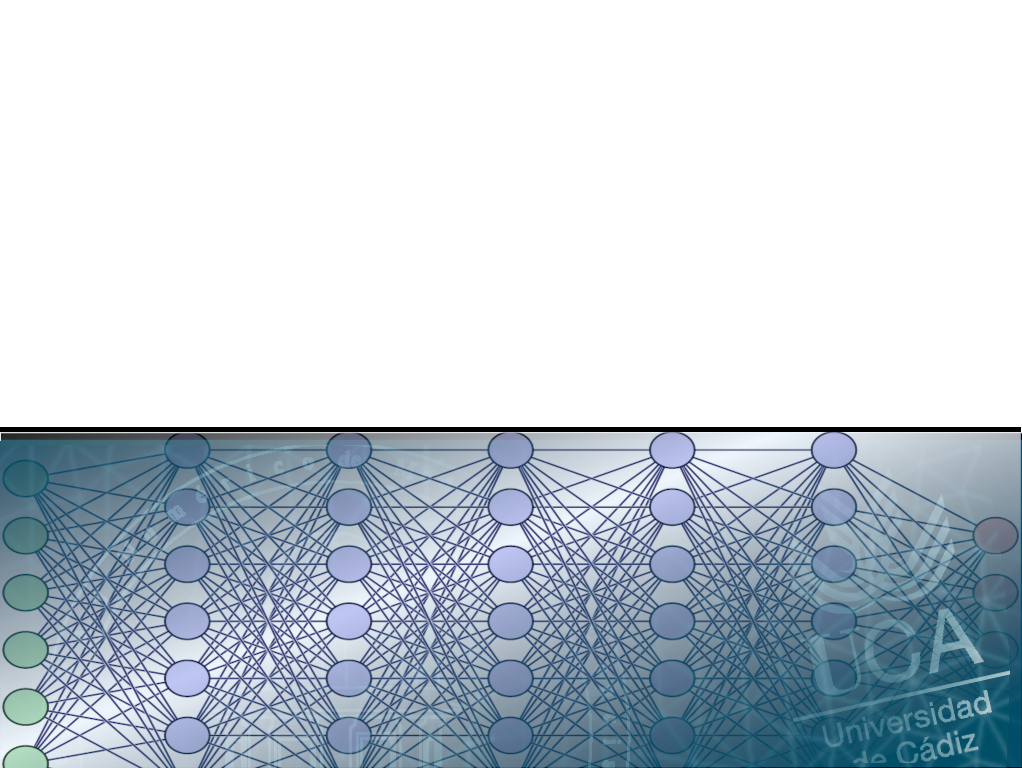
\includegraphics[width=\paperwidth,height=\paperheight]{frontpage_bg}}
\setbeamertemplate{footline}[default]
% <<<-------


% Write custom titlepage ------->>>
%\begin{frame}
%  \titlepage
%  \vspace{5cm}
%\end{frame}

% Set the background for the rest of the slides.
\setbeamertemplate{background}{}
 % {
\includegraphics[width=\paperwidth,height=\paperheight]{slide_bg}}


% Write all of the slides..........

% \begin{frame}{Outline}
%   \tableofcontents
% \end{frame}

% Start inserting infoline at the end
\setbeamertemplate{footline}[PHDtheme]
% <<<-------

%\newcommand{\imgdir}{Undefined, use renewcommand!}

%============================================================================
\section{Migración de neuroblastos en el cerebro adulto}
%============================================================================

%=====================================================================
\begin{frame}{¿Qué queremos modelar?}
%---------------------------------------------------------------------
\only<1>{
  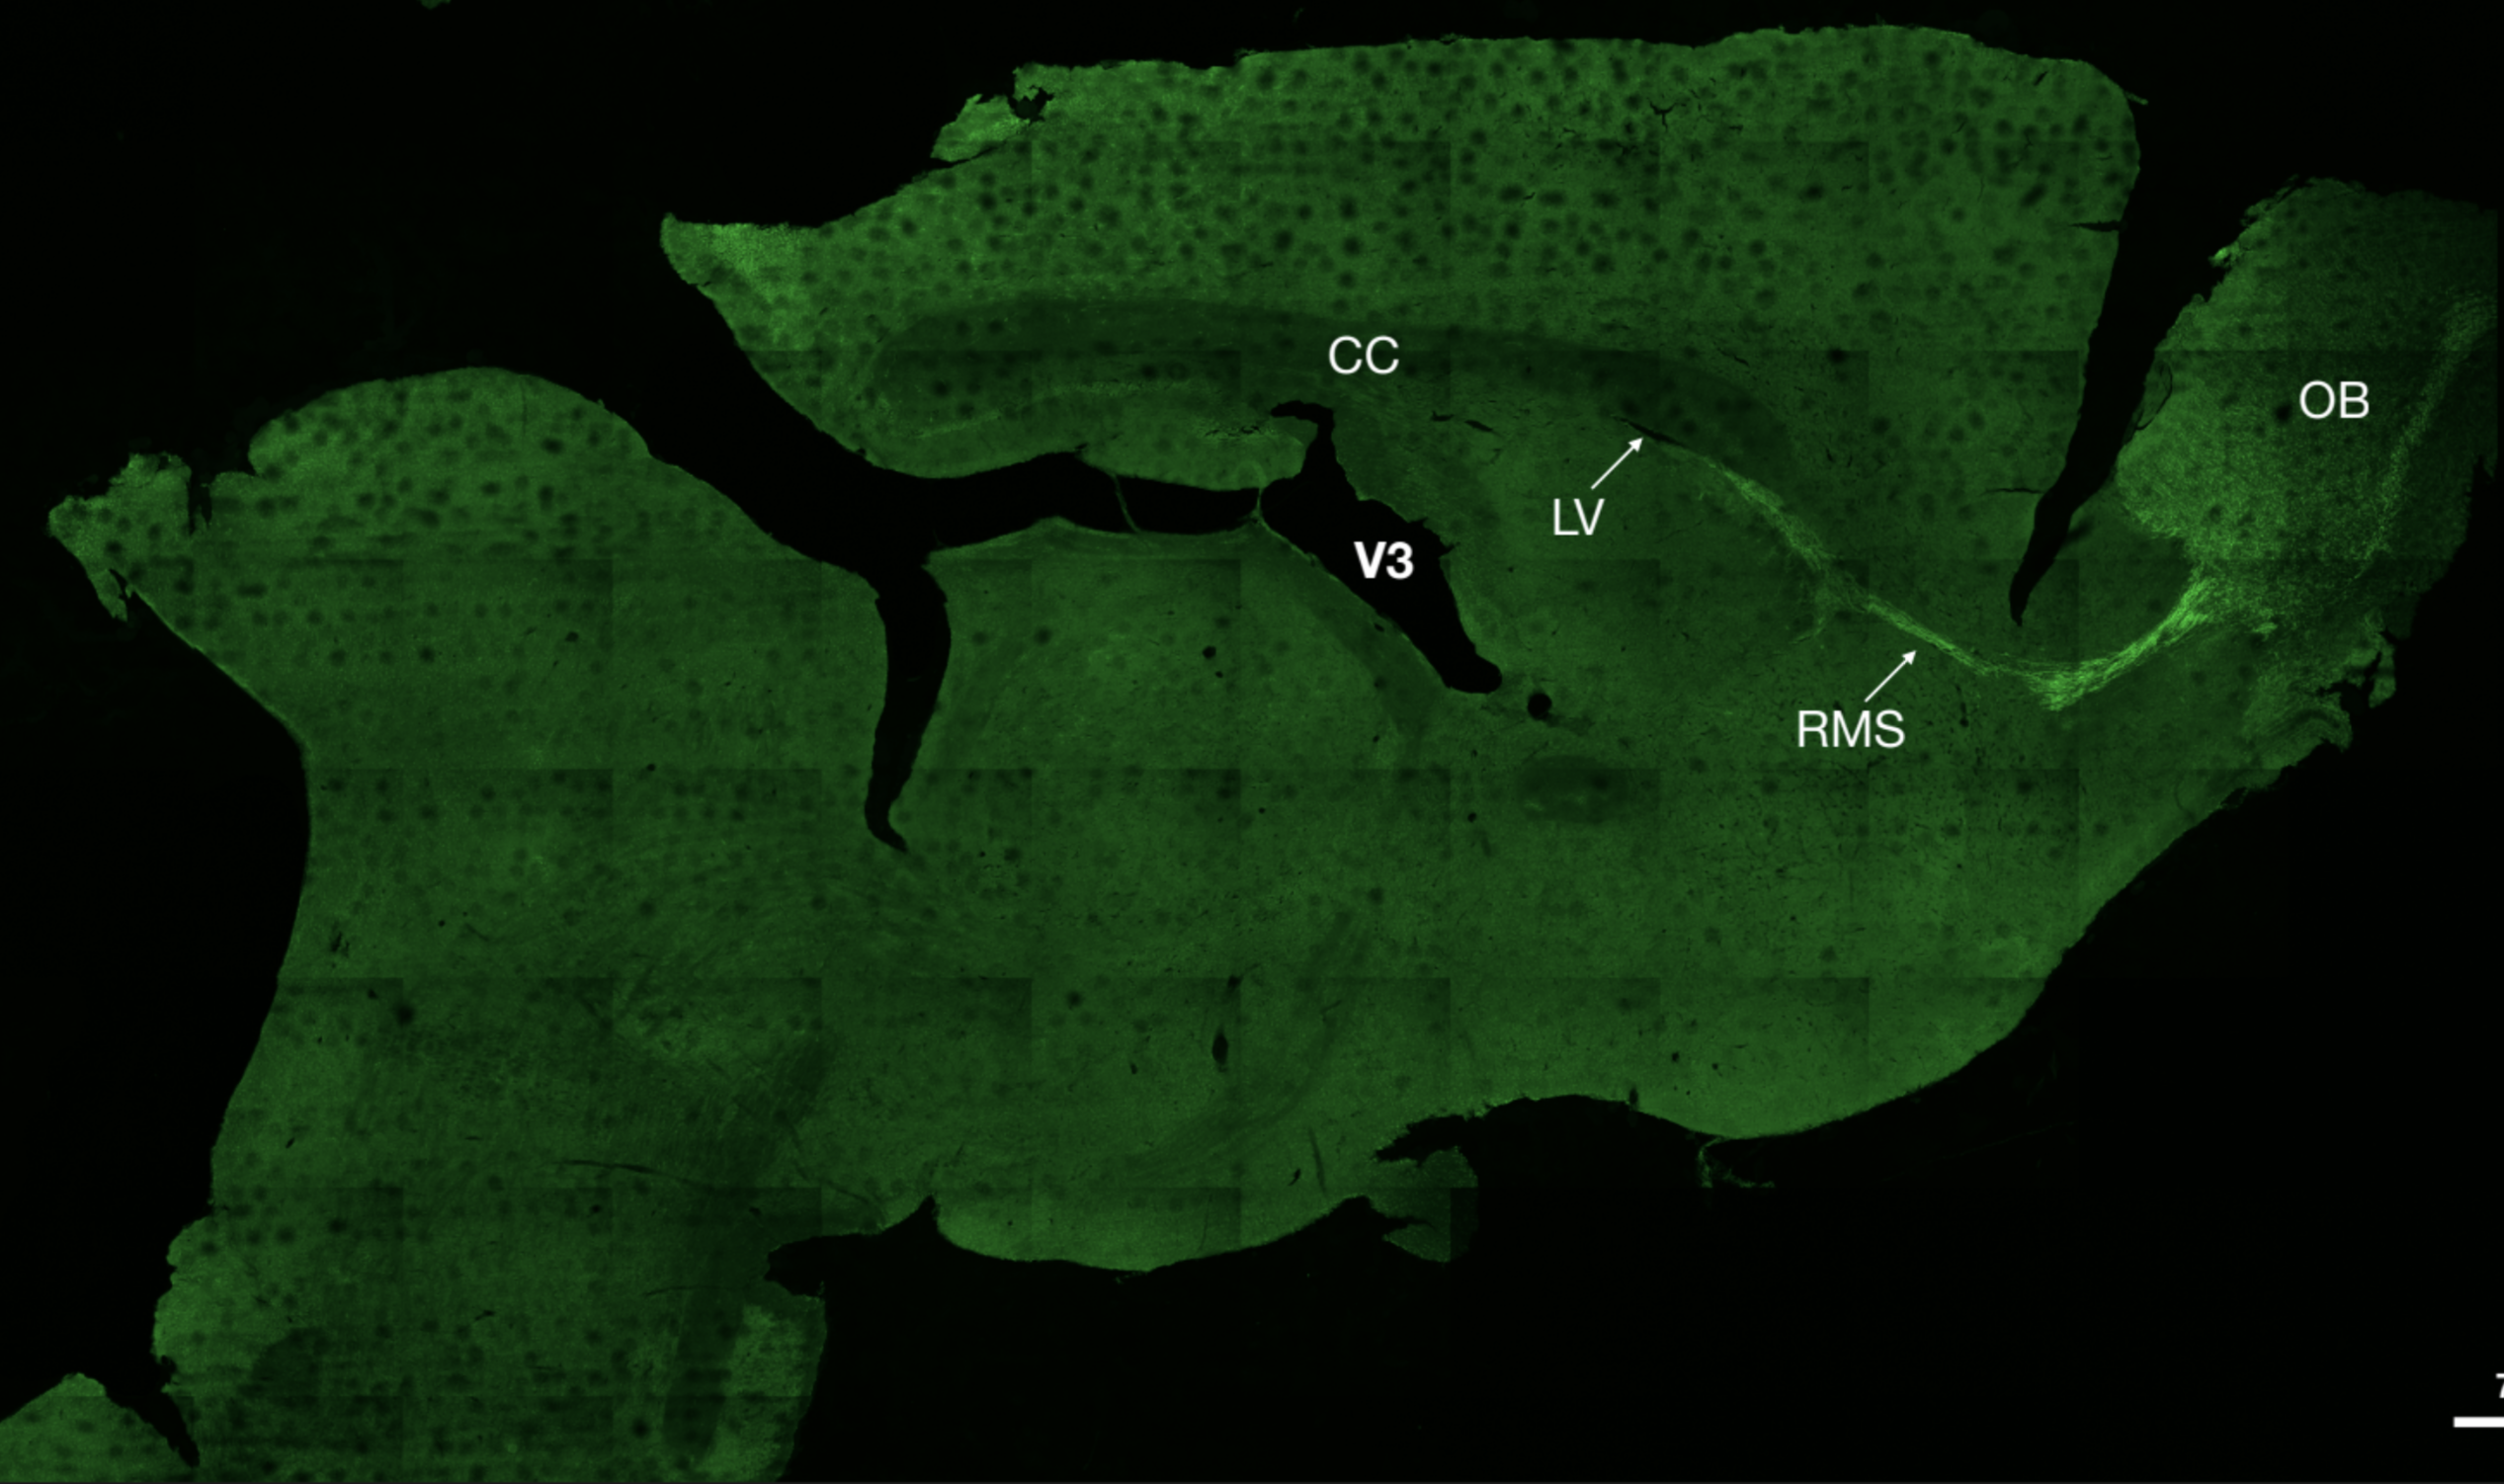
\includegraphics[width=0.95\linewidth]{cerebro-completo}}
  \only<2->{
  \includegraphics[width=0.95\linewidth]{via-rostral}}
\end{frame}

\begin{frame}{Primer objetivo: recuento de neuroblastos}
  \only<1>{
  	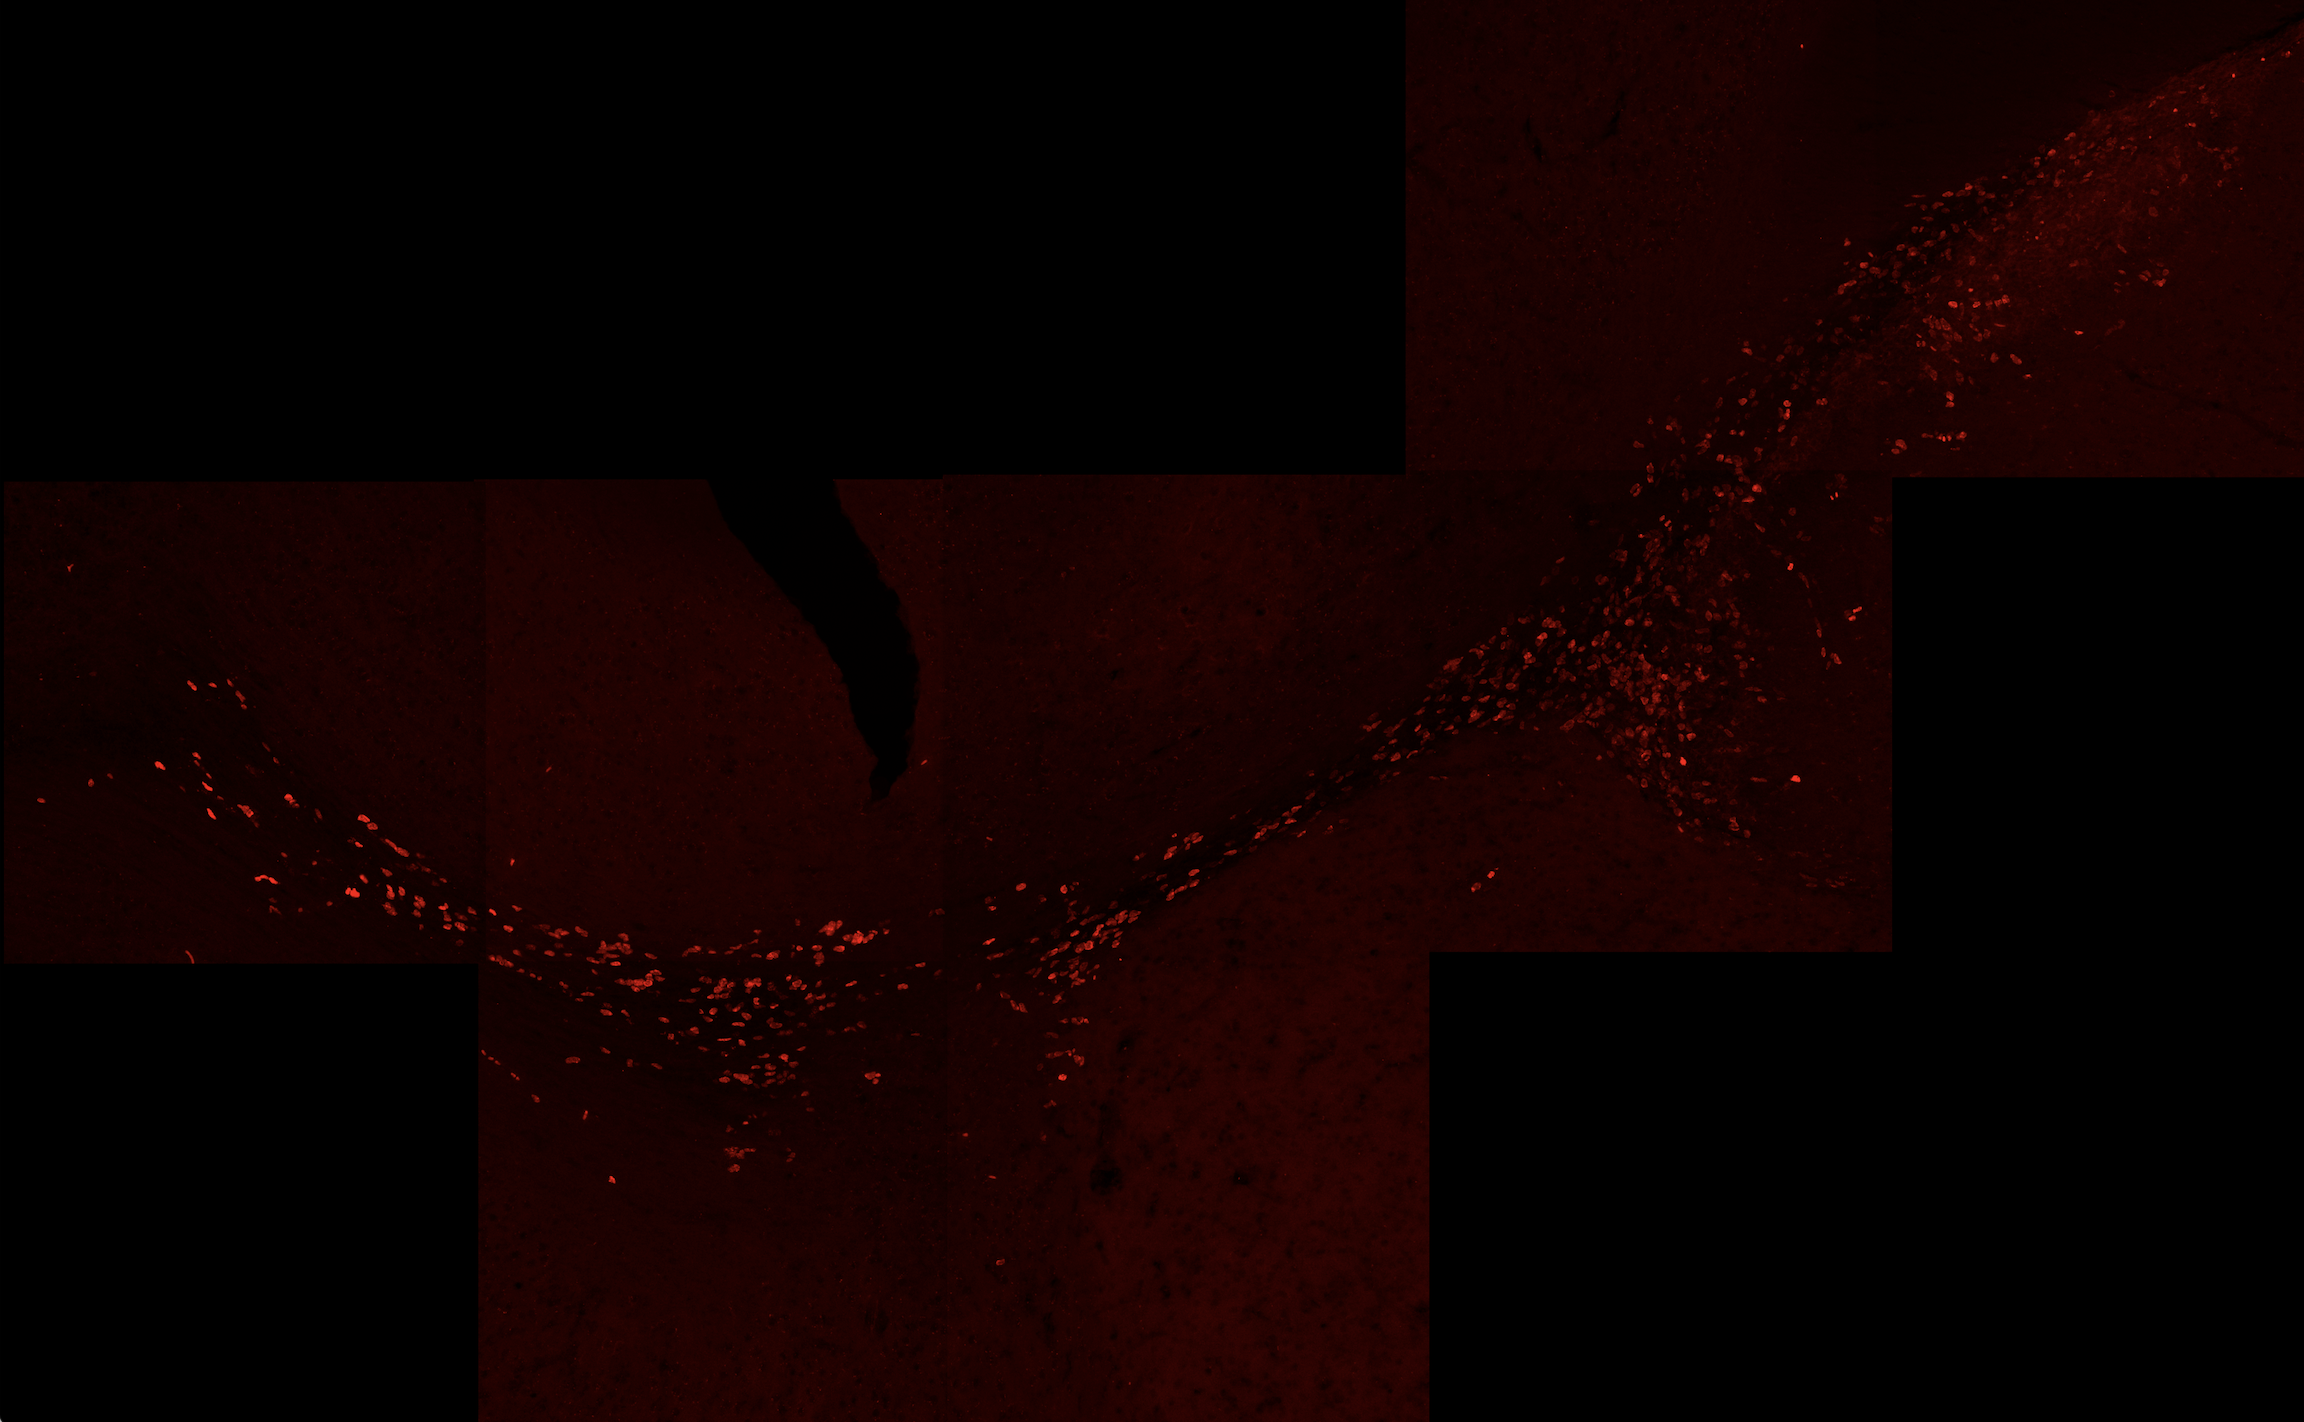
\includegraphics[width=0.95\linewidth]{via-roja}}
  \only<2->{
  	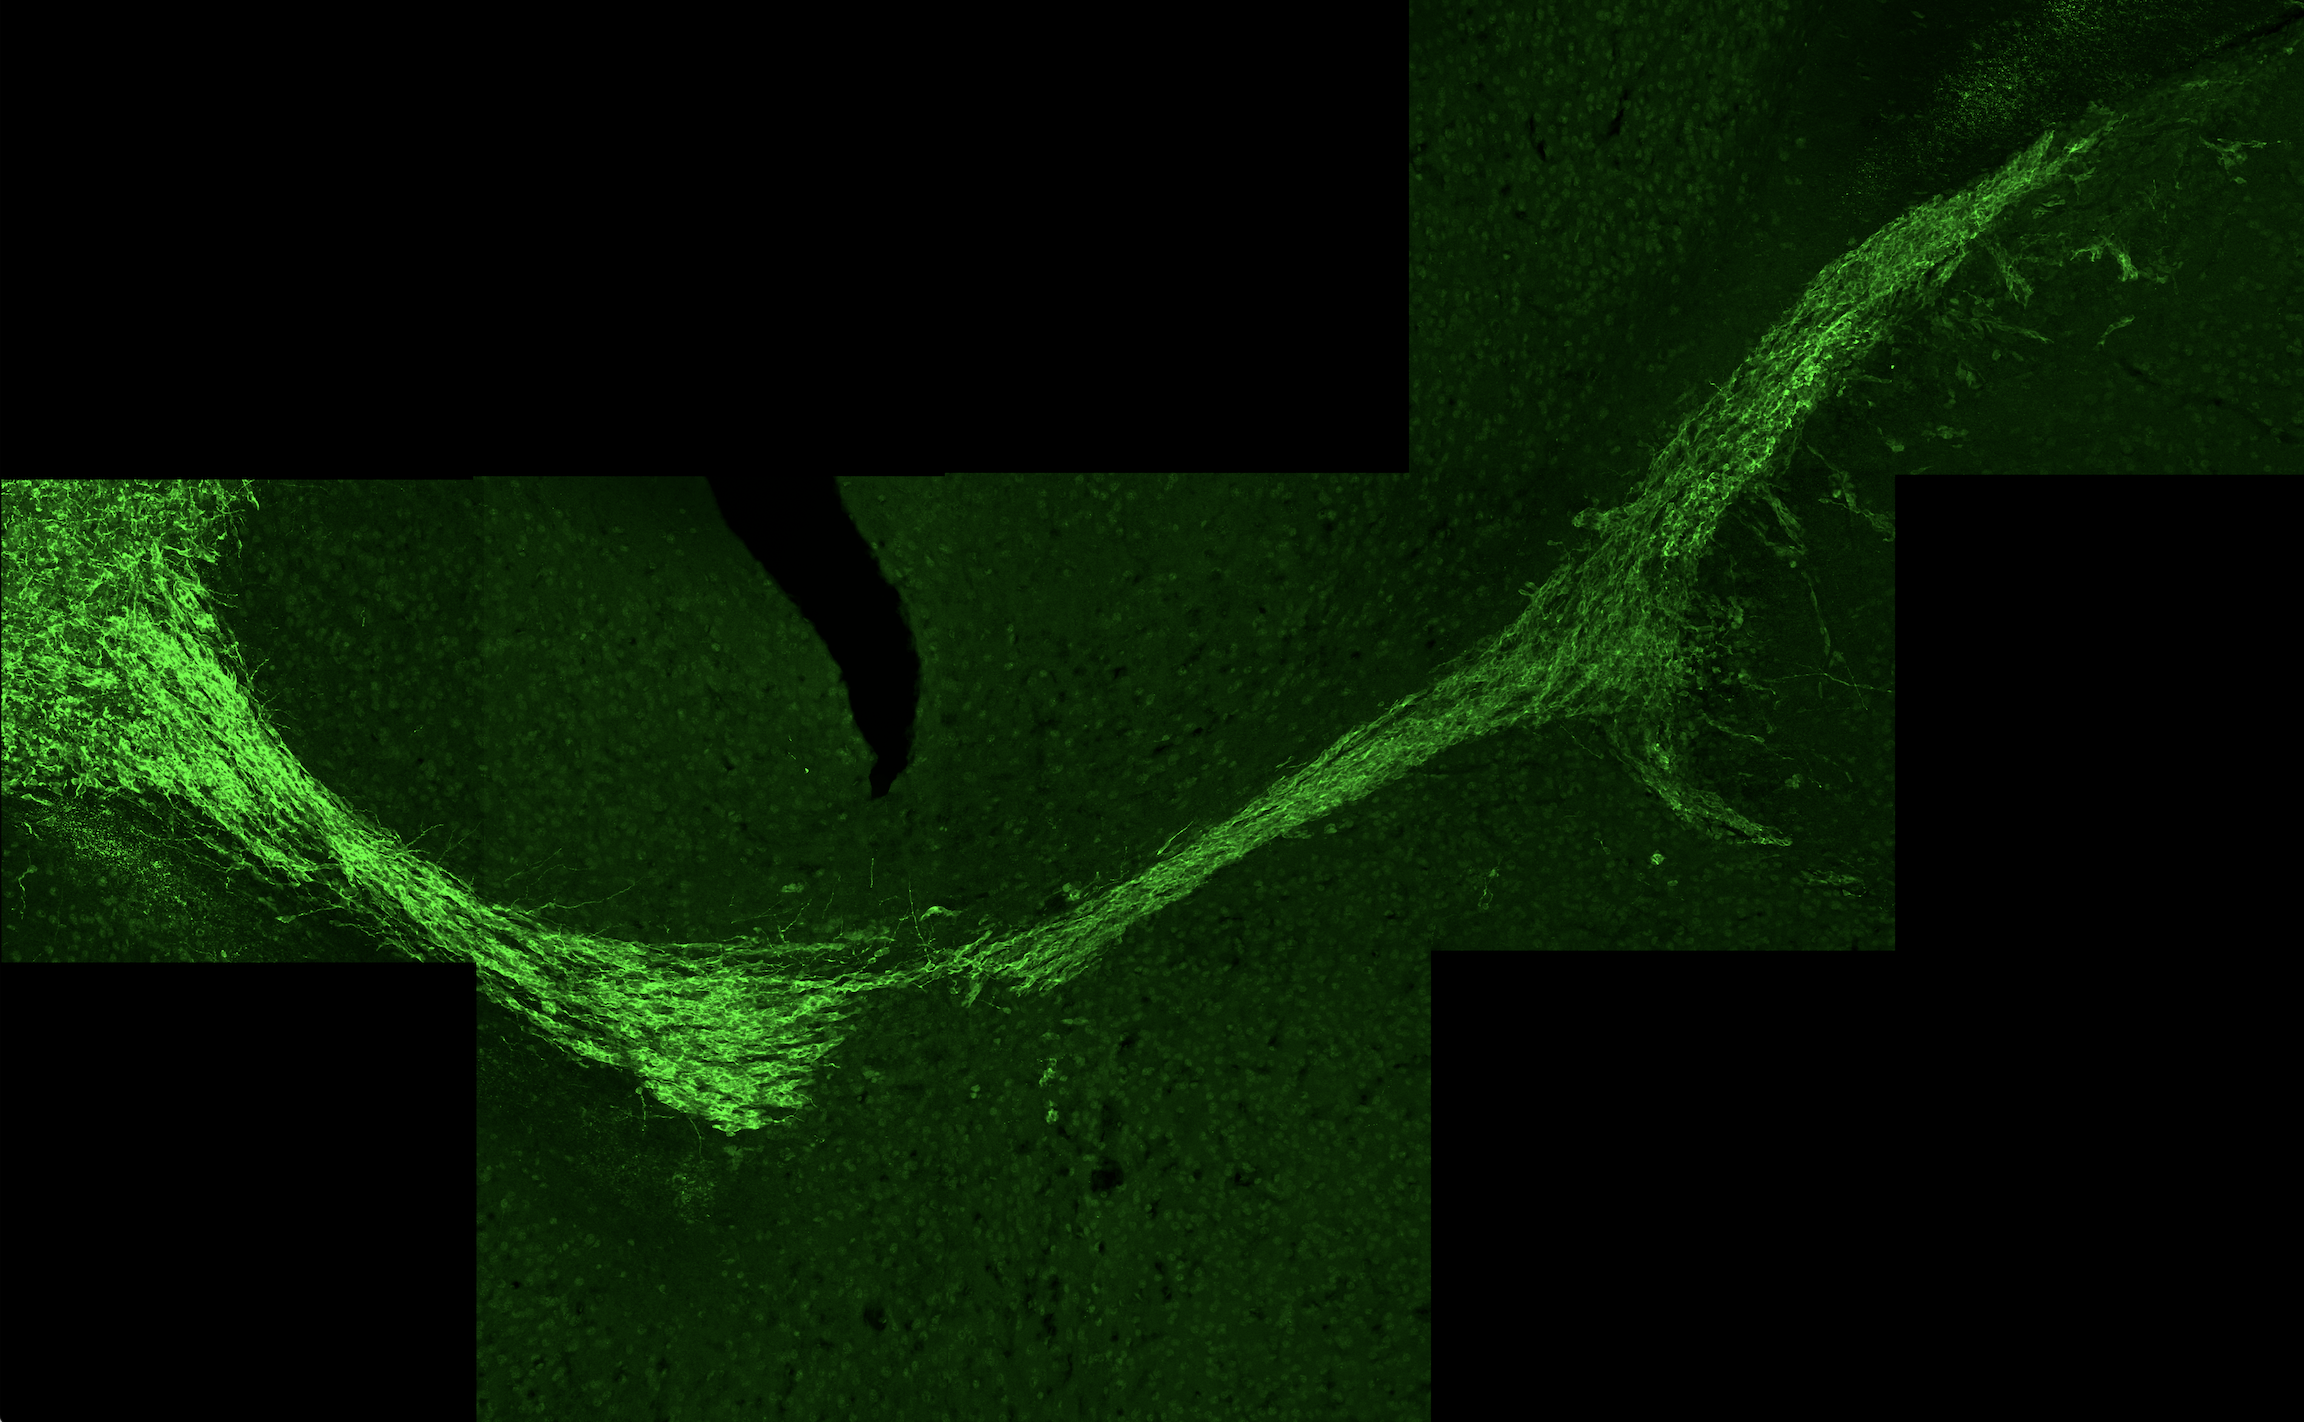
\includegraphics[width=0.95\linewidth]{via-verde}}
\end{frame}

\begin{frame}{Segundo objetivo: modelización y ajuste de parámetros}
	\begin{equation}
	\label{eq:neuroblast}
	\tau u_t + \X\, \nabla \cdot(u\nabla \O) + \alpha\, u - \gamma\, u \,1_{\NZdomain} 
	= \beta\, 1_{\SVZdomain}  
	\qquad\text{in}\enspace\Omega\times [0,T],
	\end{equation}
	\vspace{3mm}
	\begin{equation}
	\label{source}
	f_{\O}(x,y) = f_{\O}(\SO; x,y) 
	=  e^{((x-x_O)^2 + (y-y_O)^2)/\SO^2}.
	\end{equation}
	\vspace{3mm}
	\begin{equation} 
	\label{ob}
	\left\{ \begin{aligned} \Olf-\nabla\cdot (\mu_\CCdomain\,\nabla \Olf) &= f_{\O}  \quad  \text{ in } \Omega, \\
	\Olf &= f_{\O}  \quad \text{ on } \partial\Omega.
	\end{aligned}
	\right.
	\end{equation}
\end{frame}

\begin{frame}{Cerebro virtual}
	Malla
	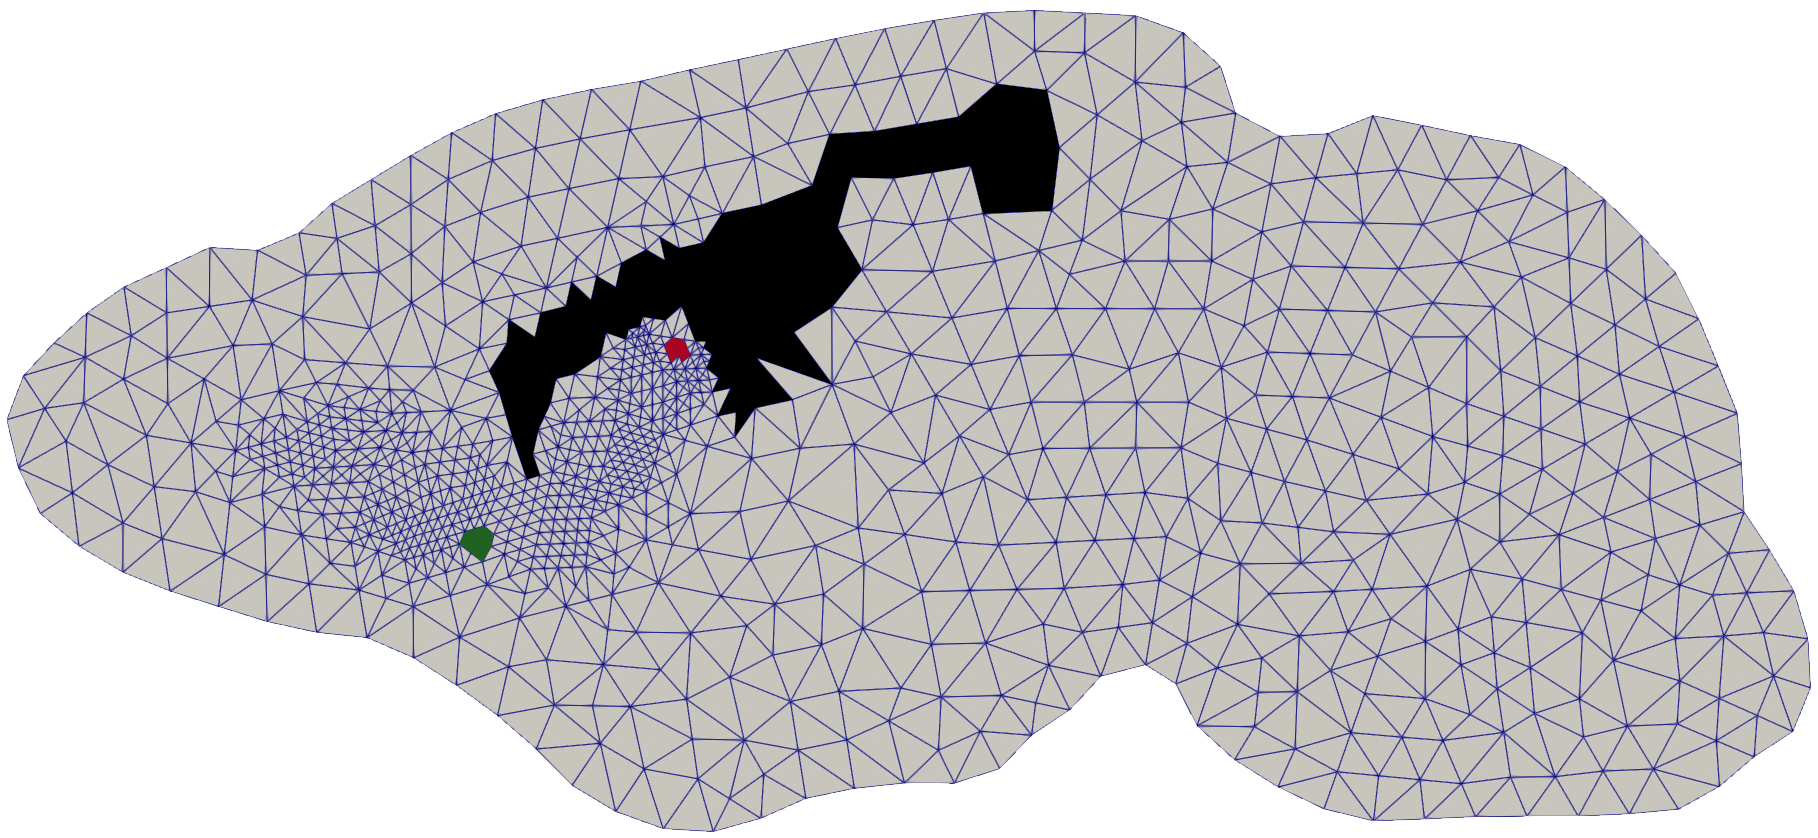
\includegraphics[width=0.95\linewidth]{brain-mesh.png}
\end{frame}

\begin{frame}{Modelización de la atracción}
Gradiente del bulbo olfatorio: parámetro $\sigma$
 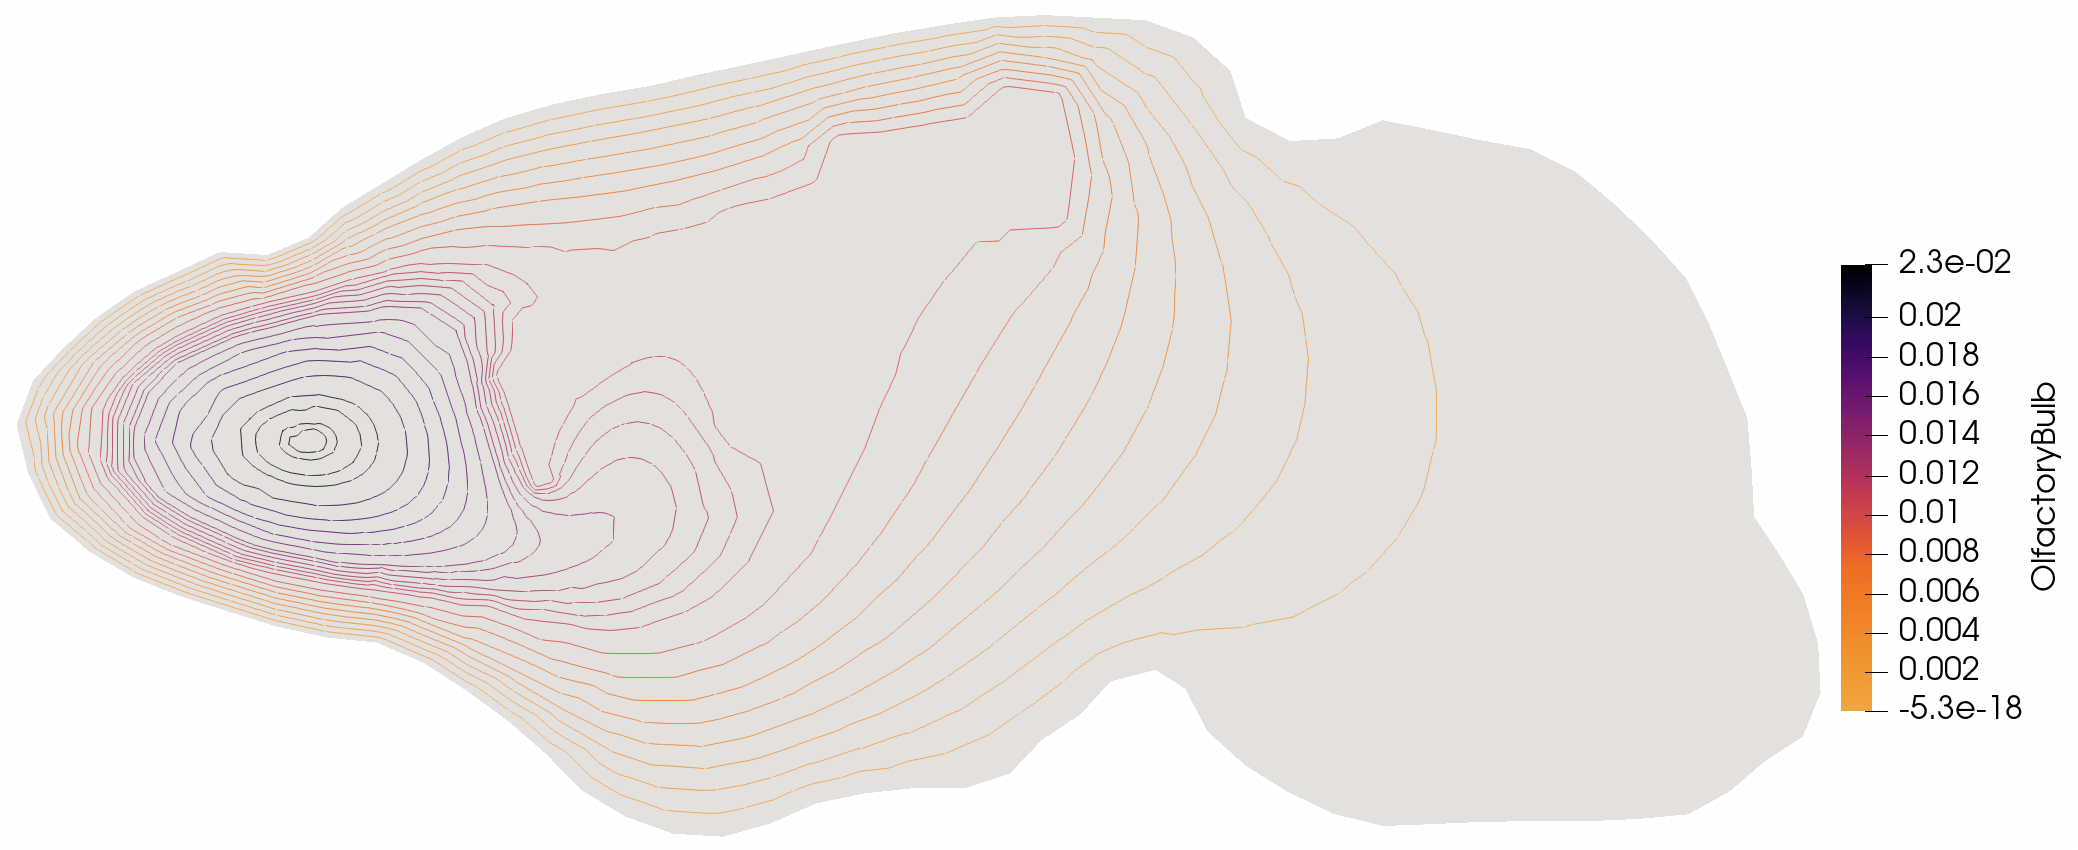
\includegraphics[width=0.95\linewidth]{ob.png}
\end{frame}
\begin{frame}{Modelización del movimiento}
	Vía rostral: parámetros $\alpha, \beta, \X, \gamma$
	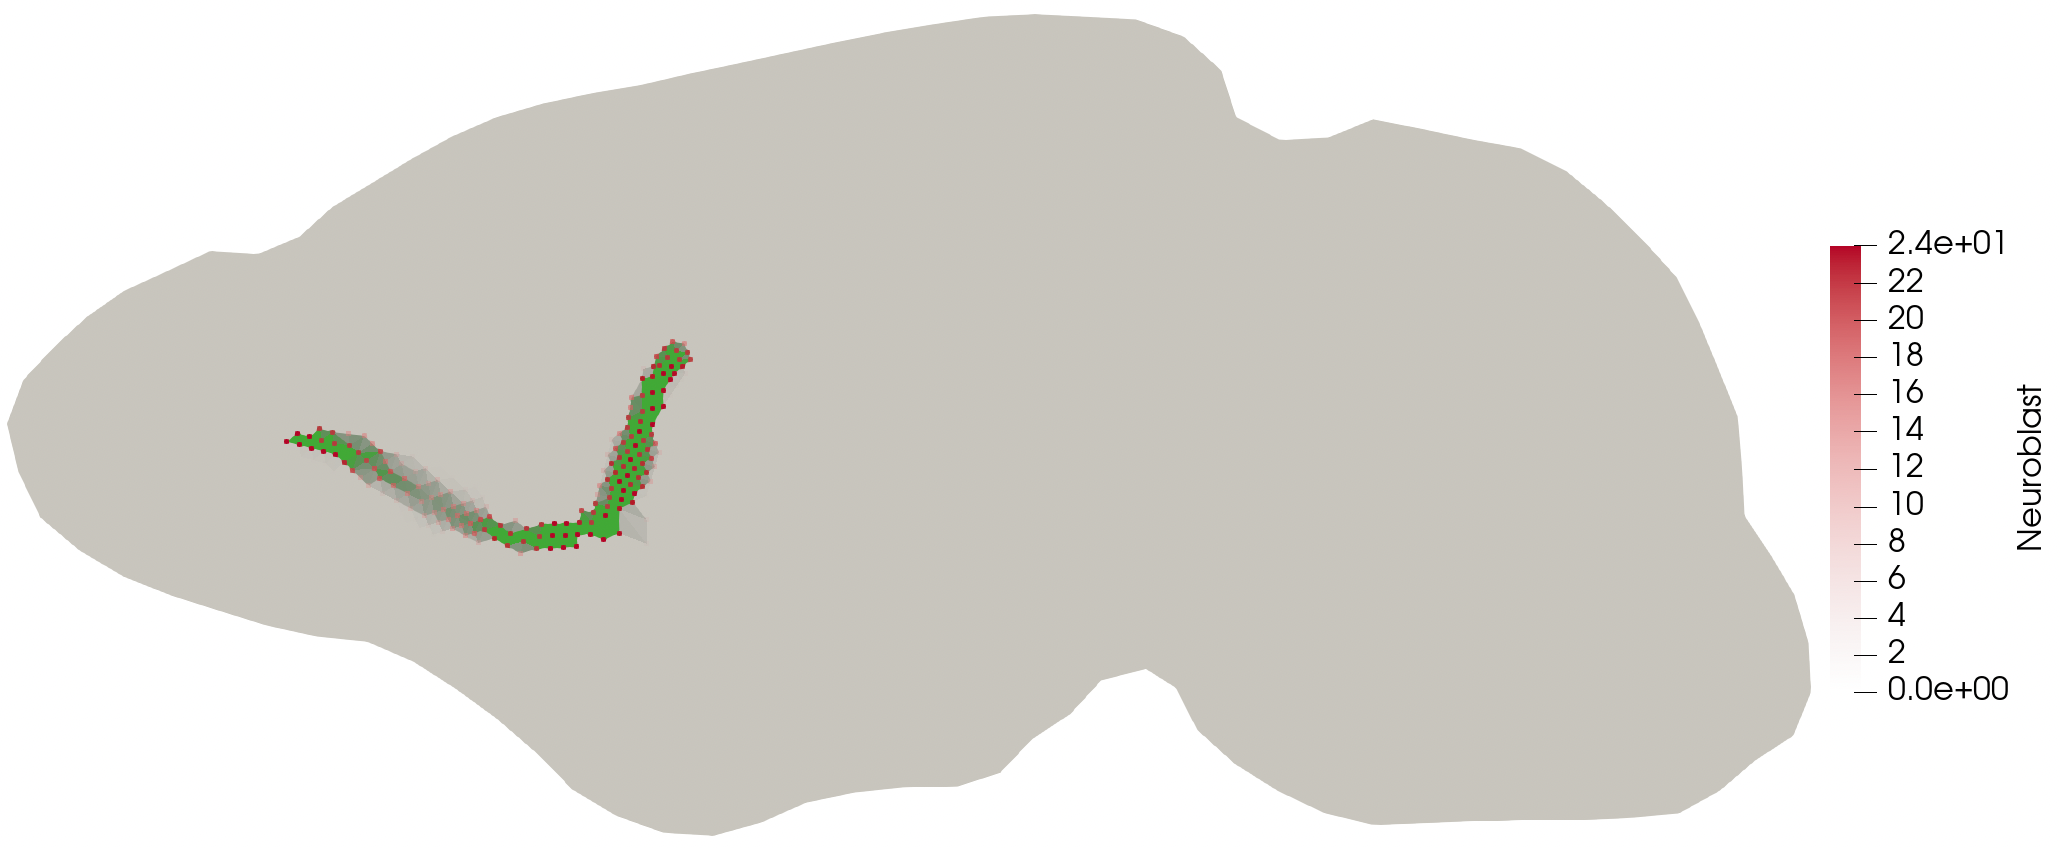
\includegraphics[width=0.95\linewidth]{steady-opt.png}
\end{frame}




%\include{dan1}
%\include{noelia}
%\include{dan2}


%\include{dan2}


%\include{dan2}


\include{dan2}

\end{document}


%%% Local Variables:
%%% coding: utf-8
%%% TeX-master: t
%%% mode: latex
%%% ispell-local-dictionary: "english"
%%% End:
